\documentclass[11pt,letterpaper]{article}
\usepackage[margin=0.93in,top=0.88in,bottom=0.91in,headheight=15pt,headsep=16pt,footskip=30pt]{geometry}
\usepackage{amsmath,amssymb,amsthm,booktabs,tabularx,array}
\usepackage{microtype,xcolor,tikz,fancyhdr,titlesec}
\usepackage[bookmarksnumbered,colorlinks=true,linkcolor=teal!50!black,citecolor=teal!55!black,urlcolor=teal!50!black]{hyperref}
\hypersetup{pdftitle={Knot theory in intuitionistic primitive recursive arithmetic},pdfauthor={ChatGPT},pdfsubject={Constructive knot theory, rational polyhedra and finite diagram invariants}}
\definecolor{ink}{HTML}{152D3C}
\definecolor{sea}{HTML}{116769}
\titleformat{\section}{\Large\bfseries\color{ink}}{\thesection}{0.58em}{}
\titleformat{\subsection}{\large\bfseries\color{ink}}{\thesubsection}{0.52em}{}
\setcounter{tocdepth}{1}
\setlength{\emergencystretch}{2em}
\setlength{\parskip}{2.8pt plus 0.5pt minus 0.4pt}
\setlength{\parindent}{1em}
\pagestyle{fancy}\fancyhf{}
\lhead{\small\sffamily\color{sea}Knot theory in iPRA}
\rhead{\small\sffamily\color{ink}Finite constructions and proofs}
\cfoot{\small\sffamily\thepage}
\renewcommand{\headrulewidth}{0.3pt}
\raggedbottom
\newtheorem{theorem}{Theorem}[section]
\newtheorem{lemma}[theorem]{Lemma}
\newtheorem{proposition}[theorem]{Proposition}
\newtheorem{corollary}[theorem]{Corollary}
\theoremstyle{definition}\newtheorem{definition}[theorem]{Definition}
\theoremstyle{remark}\newtheorem{remark}[theorem]{Remark}
\newcommand{\wiki}[2]{\href{https://en.wikipedia.org/wiki/#1}{#2}}
\newcommand{\repo}[2]{\href{https://github.com/VladimirReshetnikov/ProveIt/blob/6d03f3643ebb91a6243eb1e35e7599b388197786/#1}{#2}}
\begin{document}
\thispagestyle{empty}
\noindent{\sffamily\small\color{sea} CONSTRUCTIVE MATHEMATICS \hfill 22 NOVEMBER 2026}\par
\vspace{1.6em}
\noindent{\fontsize{24.88}{29}\selectfont\bfseries\color{ink} Knot theory in intuitionistic\\primitive recursive arithmetic\par}
\vspace{0.8em}
\noindent{\large Rational polygonal knots, diagram invariants, and proofs in Lean}\par
\vspace{1.2em}
\noindent A diagram with $c$ crossings has $2^c$ smoothing states. For a connected reduced alternating diagram, the extreme coefficients of their weighted sum survive cancellation and are $4c$ exponents apart. Every equivalent diagram must realize that span. This proves an exact crossing number by counting finitely many circles.\par
\medskip
\noindent The same arithmetic constructs a rational spanning surface for any oriented diagram and gives a sequence of at most $N-1$ triangle moves that unties any $N$-edge polygon in four dimensions. The proofs quantify over finite codes, construct witnesses, and identify the assertions used in induction.\par
\vspace{1em}
\begin{center}
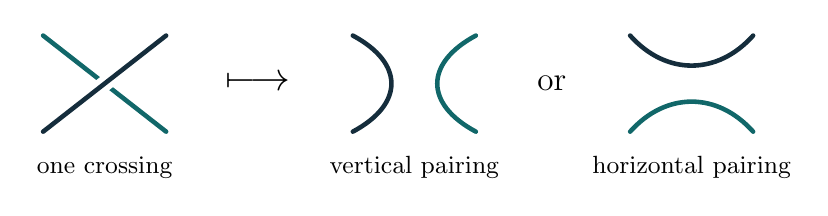
\begin{tikzpicture}[x=1.42cm,y=1.13cm,line cap=round]
\begin{scope}
\draw[sea,line width=1.65pt] (-.55,.54)--(.55,-.54);
\draw[white,line width=5.7pt] (-.55,-.54)--(.55,.54);
\draw[ink,line width=1.65pt] (-.55,-.54)--(.55,.54);
\node[font=\small] at (0,-.94) {one crossing};
\end{scope}
\node[font=\Large] at (1.37,0) {$\longmapsto$};
\begin{scope}[shift={(2.77,0)}]
\draw[ink,line width=1.65pt] (-.55,.54) .. controls (-.09,.23) and (-.09,-.23) .. (-.55,-.54);
\draw[sea,line width=1.65pt] (.55,.54) .. controls (.09,.23) and (.09,-.23) .. (.55,-.54);
\node[font=\small] at (0,-.94) {vertical pairing};
\end{scope}
\node[font=\large] at (4.0,0) {or};
\begin{scope}[shift={(5.25,0)}]
\draw[ink,line width=1.65pt] (-.55,.54) .. controls (-.23,.09) and (.23,.09) .. (.55,.54);
\draw[sea,line width=1.65pt] (-.55,-.54) .. controls (-.23,-.09) and (.23,-.09) .. (.55,-.54);
\node[font=\small] at (0,-.94) {horizontal pairing};
\end{scope}
\end{tikzpicture}
\end{center}
\vspace{.4em}
\noindent\textbf{Three distinguishing calculations.}
Here $F_q$ counts Fox colorings modulo $q$. The last column gives the minimum number of crossings among equivalent diagrams.
\begin{center}
\renewcommand{\arraystretch}{1.18}
\begin{tabular*}{0.94\linewidth}{@{\extracolsep{\fill}}lrrrr@{}}
\toprule Diagram & Components & $F_3$ & $F_5$ & Crossings\\\midrule
Trefoil & 1 & 9 & 5 & 3\\
Figure-eight & 1 & 3 & 25 & 4\\
Borromean rings & 3 & 3 & 5 & 6\\\bottomrule
\end{tabular*}
\end{center}
\vfill
{\noindent\small\textbf{Verification.} The report supplies human proofs, four standalone checked Lean modules, a ProveIt integration file, and exact computations. Section~\ref{sec:lean} gives the verification level of each. The passage from arbitrary tame ambient isotopies to diagram movies is used externally.\par}
\newpage
\tableofcontents
\vspace{1em}
\paragraph{Reading the examples.}
For the trefoil, Section~\ref{sec:fox} counts nine tricolorings, Section~\ref{sec:bracket} distinguishes its two handednesses, and Section~\ref{sec:alex} calculates its group and Alexander polynomial. For the Borromean rings, Section~\ref{sec:linking-surface} proves that all two-component sublinks are trivial while the full link has crossing number six. Section~\ref{sec:scope} maps the results back to the requested articles.
\newpage
\section{What is a knot statement in first-order arithmetic?}
The objects quantified over in this paper are natural numbers. A diagram is a code $D$, a move is finite data, and a proof that two diagrams represent the same diagrammatic knot is a list $p$. Write
\[
 D\sim_R E\quad\Longleftrightarrow\quad \exists p\;\operatorname{Movie}(D,E,p)=1.
\]
Thus an obstruction has the strong form $I(D)\ne I(E)\Rightarrow
\forall p\,\operatorname{Movie}(D,E,p)=0$. It applies to lists of every length.
A positive construction supplies the code of its witness. An integer, polynomial, group presentation, surface or embedding below always has a specified finite representation.

\paragraph{The arithmetic.}
We use intuitionistic first-order arithmetic with equality, successor axioms, defining equations for primitive recursive (PR) functions, and induction on quantifier-free formulas with parameters. These are precisely the conventions in ProveIt's \texttt{ConciseIPRA/PR.lean} \cite{proveit}. Concretely, pair $a,b$ by $2^a(2b+1)$, with $0$ reserved for the empty list. The projections on positive codes use at most the code many divisions by two. Nest pairs to code lists. Length, lookup with default zero, append, scan and reversal are obtained by loops bounded by the code or length. Arrays of fixed length $l$ with entries $<b$, $b\ge2$, can instead use $l$ base-$b$ digits. Integers are pairs modulo $(u,v)=(u',v')$ iff $u+v'=u'+v$, normalized by truncated subtraction. Rationals have a signed numerator and positive denominator, with order by cross multiplication. Laurent polynomials have an integer low exponent and a list of coefficients, trimmed at the two ends, with a separate zero flag. Addition aligns windows, multiplication is finite convolution. Every algorithm has a default result on a malformed input.

\begin{lemma}[Bounded induction interface]\label{lem:interface}
Bounded conjunction, disjunction, search with a default, double counting of a finite relation and induction over the prefixes of a supplied list can all be used with quantifier-free induction in iPRA.
\end{lemma}
\begin{proof}
For a Boolean $b(i,x)$ iterate $U(0)=1$, $U(k+1)=U(k)b(k,x)$ and $S(0)=0$, $S(k+1)=S(k)+(1-S(k))b(k,x)$. At a failure of $U$ or success of $S$, a simultaneous register stores the first responsible index; a bounded prefix check verifies the answer. Substitution of an arbitrary bounded index into a successful $U$ is proved by induction on the prefix with that index as a parameter. Conversely, to prove $U=1$ from all its instances, the induction formula is $U(k)=1$ under the given premise. Iterate these translations from the innermost bound out. A finite bijection preserves counts by summing its $0,1$ graph by rows and columns. The interchange follows by two inductions on the side lengths and distributivity of addition. On a fixed input list $p$, prove a Boolean assertion about its prefix of length $j$ by induction on $j$ with $p$ free. Checking all smaller instances uses one more bounded scan. No induction on a formula asserting unrestricted existence of a movie is needed.
\end{proof}

\paragraph{Planar input.}
Our primary input is a nonempty finite list of oriented cyclic rational polygonal curves in an oriented plane. There are no collapsed edges, nonincident vertex contacts, overlapped edges or triple points. The only self-contacts and mixed contacts outside consecutive endpoints are transverse double points in edge interiors. A bit at each records which branch lies higher. Crossings are detected by solving two affine linear equations for parameters strictly between zero and one. We allow extra subdivision vertices. A circle without crossings carries its own component record. The same algorithm handles diagrams drawn in a rectangular chart on the sphere; the outside face can be changed by redrawing the chart with a certificate.

A compact version numbers the four darts at each crossing in counterclockwise order, alternately over and under. External edges pair the darts, and an orientation chooses an incoming end on each passage. Store isolated circles separately. Following the opposite dart, then its external edge, traces a component. Using adjacent darts instead gives either smoothing. Components can be counted by marking new orbits and following each for at most the number of darts; for an unoriented pairing graph use its connected components, or count just one direction of each orbit. ProveIt's \texttt{diagram.py} uses the same local convention with the understrand in positions zero and two and checks the face permutation of a connected knot \cite{validator}. A planar drawing supplies a realizability certificate for our inputs, including the relative placements of disconnected pieces. A bare word of crossing visits need not have such a drawing.

\paragraph{Local certificates.}
A redraw supplies an orientation-preserving combinatorial isomorphism of subdivided planar cells containing the drawing, including the unbounded face and the nesting of disjoint curves. One concrete format uses a bounding polygon with oriented triangulations, a correspondence of all oriented triangles preserving incidences, and the subset of edges representing the subdivided drawing. Empty circles are retained. Triangulation validity is checked by pairwise intersection, oriented triangle areas and boundary coverage (the sum of the areas equals the bounding area). A supplied common subdivision permits coordinates to change. A disk replacement cuts out a polygonal disk whose boundary meets the drawing in the prescribed, cyclically ordered ends. With the outside fixed, a local drawing is recorded by its crossings, pairing, boundary order, overpasses and oriented incidences. Accept it by a planar-cell isomorphism to the relevant template up to subdivision. Templates are a simple strand versus a one-crossing curl (I), two disjoint arcs versus an empty bigon with one arc over at both crossings (II), and a triangular exchange of three arcs at distinct height ranks (III). Reflections, rotations, reversals of arc directions and both directions of the replacement are included. In III each pair meets once, with the same pairwise overpass before and after, and the order along each arc reverses. All certificates can use maps to a common triangulated disk with boundary marked. Thus no search for a continuous homeomorphism enters the verifier. On a single crossing the usual sign is fixed by the positive Artin braid generator; mirroring interchanges the signs.

\begin{proposition}[Certificate calculus]
Diagrammatic equivalence is reflexive, symmetric and transitive. Component count is invariant. If a PR observable agrees under a local move and redraw, it agrees along every accepted movie. For any numerical bound $B$, the existence of a movie whose whole code is at most $B$ is decidable in iPRA.
\end{proposition}
\begin{proof}
Use an empty list, reverse the moves and their local isomorphisms, or concatenate lists. Tracing a boundary end through each of the six local tangles gives the same exit before and after; no closed component lies entirely in a moving tangle. Thus the external successor cycles and the isolated components have the same count. For an observable $I$, scan $p$ with prefix invariant $I(D_j)=I(D_0)$, under the fixed assumption of acceptance. For a given $B$ apply the bounded search of Lemma~\ref{lem:interface} to codes $0,\ldots,B$. This proves no bound on the smallest witness as a function of the endpoints.
\end{proof}

\paragraph{Classical interpretation.}
The classical Reidemeister theorem identifies the diagram quotient with tame link types up to ambient isotopy \cite{rei,kauffman}. We use it to identify the conventional topological reading of the diagram theorems. Its full completeness assertion for arbitrarily presented isotopies is external here. The arithmetic conclusions on move lists and the geometric constructions in the next section have independent proofs.

\section{Polygonal knots in three and four dimensions}
\label{sec:geometry}
A polygonal link is a list of cyclic lists of rational points. Each circuit has at least three edges. Adjacent edges meet precisely at their common endpoint; all other edges are disjoint. In dimension $d$, an elementary triangle move replaces one side of a nondegenerate rational triangle by the other two or vice versa, when the triangle meets the rest of the polygon only in the permitted endpoints. Subdivision and its inverse are allowed. These are assertions about finite lists. Intersections of rational simplices reduce to feasibility of rational linear equations and inequalities in barycentric coordinates. For a fixed ambient dimension and simplex size, eliminate one variable at a time by combining every lower bound with every upper bound; retain the open/closed flags if a facet is excluded. Given values for the remaining variables, back-substitute a midpoint between bounds, the common value of two closed equal bounds, or a point one unit beyond a one-sided bound. This proves both the test and rational witness property. In particular disjointness is a decidable arithmetic predicate.

\begin{lemma}[Finite grid avoidance]\label{lem:grid}
A nonzero rational polynomial of total degree at most $d$ in $k$ variables has a nonzero value on $\{0,\ldots,d\}^k$.
\end{lemma}
\begin{proof}
In one variable, division by $X-a$ with remainder $f(a)$ shows that each different root extracts a new linear factor. A polynomial having $d+1$ distinct roots and degree at most $d$ is zero. In several variables regard the last variable as the main variable. Vanishing at the entire grid forces all coefficient polynomials to vanish at every grid point in the other variables. Repeat. For its arithmetic formulation inspect the bounded grid for a witness. If none is found the coefficient argument gives a contradiction. For a varying number of variables, fix the input coefficient array and aggregate the tests on all its successive coefficient slices in a bounded conjunction. There are at most $(d+1)^k$ coefficient slots at any level. Induct on the number of coordinates eliminated with this conjunction as invariant. The projection application uses only two variables. For products we use the lexicographically largest nonzero coefficient of each factor: their product is the largest coefficient of the product. All these assertions concern finite coefficient arrays.
\end{proof}

\begin{theorem}[Regular rational projection, with a bound]\label{th:projection}
From an embedded rational polygonal link with $N$ edges in three-space one can compute $u,v\in\{0,\ldots,10(N+1)^3\}$ such that
\[
             (x,y,z)\longmapsto (x-uz,y-vz)
\]
is a regular diagram projection. Overpass bits are recovered by rational comparisons. The crossing count is at most $\binom{N}{2}$, and at most $N(N-3)/2$ for a knot.
\end{theorem}
\begin{proof}
Write $d=(u,v,1)$. We describe finitely many nonzero polynomial factors to be avoided. For a nonzero edge direction forbid collapse by taking a nonzero component polynomial of its projected direction. Do the same for differences of distinct vertices. For each nonparallel pair of supporting lines with directions $a,b$ exclude $d\cdot(a\times b)=0$. For a pair of distinct parallel lines exclude directions in their common plane of directions: its nonzero normal is $a\times(Q-P)$, where $P,Q$ are on the two lines. Collinear segments retain their separation and order whenever the common line does not collapse. For a vertex outside a supporting line forbid the plane of directions spanned by the edge and the vector from a point of the line to the vertex. A vertex on the supporting line is already handled by injectivity there. All plane factors have degree at most one and a nonzero normal gives a polynomial which is not identically zero.

Two different nonparallel coplanar lines meet in three-space. If their projections meet in segment interiors, their unique projected intersection must be the image of that very point. Since the original segments are embedded, this is impossible. Parallel pairs were handled above. Consequently a triple crossing of segment interiors can involve only three pairwise skew supporting lines. For such a triple, write the three projected line equations in homogeneous plane coordinates, each obtained as the cross product of its two projected endpoints $(x-uz,y-vz,1)$. Their three-row determinant $H(u,v)$ detects concurrence. Each row has entries affine in $(u,v)$ because the two $uv$ terms cancel, so $\deg H\le3$.

Here is why this last factor really is nonzero. Take a rational point $P$ on the first line and let $Q$ vary on the second. The plane through $P$ and line two cannot contain line three, since lines two and three are skew. In its projective completion it therefore meets line three in a single point $S$ (possibly a direction at infinity). This is just a linear equation along line three; its constant nonzero case gives its point at infinity. $S\ne P$. At most one of the lines $PQ$ passes through $S$. Choose $P$ so that the whole second line is not at its height when that line is horizontal. This is possible since two horizontal lines at the same height cannot be skew. Then at most one further $Q$ gives equal heights. Among three distinct rational $Q$'s choose one avoiding both exceptions. In the direction $Q-P$, normalized to last coordinate one, the projections of the first two lines meet transversely: coplanarity of their directions with $Q-P$ would say the lines were coplanar. The third does not collapse to a point, since a direction parallel to it would put its point at infinity on $PQ$ and in the chosen plane. The fiber $PQ$ misses line three. Hence its projected line misses the finite intersection of the first two and $H(u,v)\ne0$. This witness construction uses only affine linear equations (at most two candidate points suffice for $P$).

The sum of the degrees of these factors is bounded by $10(N+1)^3$: there are at most $N$ edges and vertices, quadratically many point/line and pair conditions, and at most $\binom N3$ determinants of degree three. Apply Lemma~\ref{lem:grid} to their product. Distinct projected intersections on one edge can now be ordered by rational edge parameter. At a crossing the original heights cannot coincide, by injectivity of the original link. Only nonadjacent edges can cross, which gives the two numerical bounds. The linear shear $(x-suz,y-svz,z)$ has an explicit inverse at every $s\in[0,1]$, giving the conventional ambient interpretation of our coordinate choice.
\end{proof}

\begin{proposition}[Lifting a diagram]
Every rational polygonal diagram in the plane has a rational polygonal link lifting it. Lifts with the same parametrized projection and the same strict height order at each crossing can be joined by a linear interpolation of heights through embeddings.
\end{proposition}
\begin{proof}
Subdivide each original edge at every crossing occurrence. Assign height $+1$ to the upper occurrence, $-1$ to the lower and $0$ to the remaining vertices. Interpolate along the subdivided edges. A coincidence in space would project to a coincidence in the plane; at the only distinct preimages of any point the heights differ. For two lifts, take a common subdivision. If the two differences of upper and lower heights are $a,b>0$, the interpolated difference $(1-s)a+sb$ is at least $\min(a,b)>0$. This proves the assertion with rational input even when reading the interpolation over real parameters. The arithmetic certificate consists of the finite list of endpoint inequalities and affine formulas.
\end{proof}

\begin{theorem}[Unknotting every polygon in four-space]\label{th:four}
A rational polygonal knot in $\mathbb Q^4$, with $N$ edges, can be changed to a triangle using at most $N-1$ elementary triangle moves. A cone point with coordinates $(t,t^2,t^3,t^4)$ exists with $0\le t\le4N^2$.
\end{theorem}
\begin{proof}
For every pair of edges, including a repeated edge, their four endpoints span an affine space of dimension at most three. By rational row reduction choose a nonzero affine linear form vanishing on that space. Its value on $(t,t^2,t^3,t^4)$ is a nonzero polynomial of degree at most four, as the five monomials are distinct. The product for at most $N^2$ forms has at most $4N^2$ distinct roots. Bounded search produces $P$ avoiding all these affine spans. Cone every edge to $P$.

Two points $x,y$ on the old polygon lying on a line through $P$ must coincide: otherwise $P$ belongs to the affine span of the edges containing them. Thus two cone triangles intersect only in their prescribed common faces, as follows by inspecting rays from $P$. Each triangle is nondegenerate. Write the vertices $v_0,\ldots,v_{N-1}$. Replace $v_0v_1$ by $v_0Pv_1$. Next replace $Pv_1v_2$ by $Pv_2$, then $Pv_2v_3$ by $Pv_3$, and continue until the boundary is the triangle $v_0Pv_{N-1}v_0$. These moves are clean by the intersection statement. There are $1+(N-2)=N-1$ moves (or keep an initial triangle). Any nondegenerate rational triangle is a standard unknotted polygon: inside its plane it bounds its filled affine disk. If one fixed standard triangle is desired, replace its vertices one at a time via auxiliary triangles as detailed below.
\end{proof}

\begin{center}
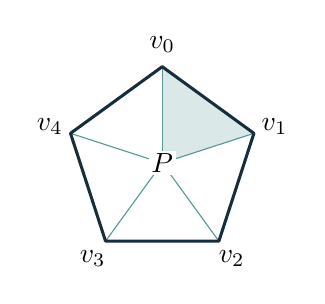
\begin{tikzpicture}[scale=.79,line join=round]
\coordinate (o) at (0,0);
\foreach \i/\a in {0/90,1/18,2/-54,3/-126,4/162}
  \coordinate (v\i) at (\a:1.55);
\fill[sea!15] (v0)--(o)--(v1)--cycle;
\foreach \i in {0,...,4} \draw[sea!70] (o)--(v\i);
\draw[ink,line width=1.1pt] (v0)--(v1)--(v2)--(v3)--(v4)--cycle;
\node[fill=white,inner sep=0.9pt] at (o) {$P$};
\foreach \i/\a in {0/90,1/18,2/-54,3/-126,4/162}
  \node at (\a:1.90) {$v_{\i}$};
\end{tikzpicture}
\end{center}
\noindent The pentagon shows the incidence pattern of the cone disk. In the shaded triangle, replace the boundary edge $v_0v_1$ by $v_0Pv_1$. Each subsequent move deletes one old vertex along an adjacent triangle. Avoidance of the edge-pair spans proves that these faces are embedded in four-space.

For this last identification there is also a direct ambient certificate. Complete the two independent side vectors to a rational basis, reversing the sign of a complementary vector if necessary to make its determinant positive. Translation followed by this change of basis takes a fixed coordinate triangle onto the given triangle. Gaussian elimination expresses a positive-determinant rational matrix as shears, positive diagonal scalings, and simultaneous sign changes on pairs of axes. A signed row exchange and a pair sign change are products of shears (in two dimensions $\left(\begin{smallmatrix}0&1\\-1&0\end{smallmatrix}\right)$ is the product of shears with successive off-diagonal entries $1,-1,1$). Each shear and positive diagonal scaling interpolates to the identity rationally without losing invertibility. For a triangle-move-only version, join the original and target triangles via a third triangle with new rational vertices chosen successively off the affine spans of every triple of already named points and off their lines. Use the moment curve test above with the degree bound four per forbidden plane. Replace vertices one at a time, first to the auxiliary triple and then to the target triple. A replacement $ABC\to A'BC$ uses two faces of the tetrahedron $AA'BC$: insert $A'$ on $AB$ by a triangle move, then delete $A$ along $CA A'$. Affine independence of every mixed quadruple used here follows from the choices of the auxiliary points (take all six old and target vertices as named at the outset; the old and target triples themselves are noncollinear). This gives an explicit connection to a fixed triangle.

\paragraph{Internal bounds.}
Solving the fixed small linear systems above uses determinants of bounded size, with signs and zero tests on integers. For the regular projection one may simply try every pair in the stated square and validate the resulting diagram. For the cone point there are $4N^2+1$ trials. To obtain the triangle-move certificate, write the remaining prefix fan after each edge: its validity is the bounded conjunction of the pairwise simplex tests. Arithmetic induction is on the number of edges already removed, with this Boolean conjunction and the explicit boundary list as invariant. No compactness or topological general-position theorem enters either construction.

\subsection{A ribbon disk gives a slice disk}
An oriented polygonal knot is \emph{PL slice}, in the sense used here, if it bounds a properly embedded rational triangulated disk in a four-dimensional box, with its boundary in the interior of a three-dimensional face. A \emph{ribbon disk certificate} is a triangulated parameter disk and a rational simplexwise affine immersion $f$ into three-space with the following recorded self-intersections. The double locus has finitely many disjoint arcs and no triple points. Each double arc has two disjoint preimage arcs mapped homeomorphically onto it, one proper (ends on the boundary) and the other entirely in the interior. These arcs are subcomplexes after a supplied subdivision, and the lists account for every coincidence of distinct points, as can be checked by triangle-pair intersections. The boundary is the prescribed knot.

\begin{theorem}[Ribbon implies slice, with an explicit fourth coordinate]
From a ribbon disk certificate one can construct a slice disk certificate by one barycentric subdivision and a vertex-height assignment.
\end{theorem}
\begin{proof}
Barycentrically subdivide the parameter disk, retaining its boundary and all the marked arcs as subcomplexes. Give height $0$ to boundary vertices, $2$ to vertices of every interior preimage arc, and $1$ to every other vertex. Extend height $h$ affinely on each small triangle. Its zero set is exactly the boundary: vertices of a barycentric simplex form a chain of nested old faces, and any face of the simplex all of whose vertices are boundary barycenters is contained in the largest boundary face in that chain. On each interior preimage arc $h=2$ everywhere. On its paired proper arc $0\le h\le1$, including at its endpoints. Thus $(f,h)$ separates every former double point, and its projection precludes any new coincidences. It gives a rational embedded triangulated disk; its inverse on each image simplex is the affine inverse furnished by the nondegenerate input triangle. Pick an integer $M$ strictly larger than every absolute coordinate of every image vertex. The disk lies in $[-M,M]^3\times[0,3]$, meets the boundary of this box exactly in the given knot at height zero, and has interior in the open box. A triangle yields six barycentric triangles, and all checks are bounded vertex, face and intersection tests. This proves the forward implication for the finite PL definitions; the converse is the slice--ribbon question, outside these proofs.
\end{proof}

\section{Descending diagrams and a constructive unknotting bound}
\label{sec:descending}

Choose a regular basepoint and a traversal direction on a one-component
diagram. The diagram is \emph{descending} if the first visit to each
crossing is on its overstrand. We shall turn this condition on the
$2c$-letter visit word into a certificate of polygonal unknotting in
three-space.

\begin{lemma}[Changing the heights of a lift]
Two rational polygonal lifts of the same parametrized regular diagram,
with the same overpass at each crossing, are related by rational
triangle moves and subdivisions in three-space.
\end{lemma}
\begin{proof}
Subdivide the two projected circuits simultaneously at all height
breakpoints and at both occurrences of every crossing. A vertex at a
crossing now has a distinct vertex of the other branch above or below it.
If a vertex $A$ with neighbors $U,V$ is moved vertically to $A'$ without
sweeping past or meeting that other branch, two triangle moves implement
the displacement. Insert $A'$ on $U A$ using the triangle $UAA'$, and
delete $A$ from $A'AV$ using the triangle $A'AV$. Skip zero displacements.
Both triangles are nondegenerate: the neighboring projections are
different from that of $A$. Each projects onto one incident projected
halfedge. Its open projected halfedge contains no other branch, by the
subdivision. Over the moved vertex the triangle occupies precisely the
interval of heights being swept; over the other endpoint it occupies
just the unchanged endpoint. The two incident halfedges have disjoint
interiors. These observations verify the clean-triangle tests, including
when a neighboring vertex is another crossing occurrence.

At each crossing first move the upper vertex to the larger of its
initial and target heights and the lower to the smaller of its two
heights. Then move them to their target heights. The
upper vertex can be moved first, since its target is strictly higher
than the target lower height and than the temporarily lowered vertex.
The lower vertex can then be moved. Every intermediate comparison is
strict. Move ordinary vertices once to their targets. This gives at most
four triangle moves per common-subdivision vertex.
\end{proof}

\begin{theorem}[A descending diagram bounds a polygonally unknotted lift]
Every rational polygonal lift of a descending diagram admits a finite
rational triangle-move sequence to a triangle. Both a lift and such
a sequence are primitive recursively constructible.
\end{theorem}
\begin{proof}
Take the basepoint $b$ in the interior of an edge, and choose points
$b^-,b^+$ immediately before and after it in traversal order.
The short interval from $b^-$ to $b^+$ contains no crossing, bends or
other passages of the diagram. Its endpoints can be chosen by taking
midpoints to the nearest recorded event on either side along that edge.
Subdivide at these two points, all old bends and all crossing occurrences.
Read the resulting planar list from $b$ back to $b$ as
$p_0,p_1,\ldots,p_m$, with $p_0=p_m=b$, $p_1=b^+$ and $p_{m-1}=b^-$.
Choose strictly decreasing heights $z_i=m-i$ and put
$A_i=(p_i,z_i)$ and $B_i=(b,z_i)$. First form the temporary polygon
consisting of the chain $A_0\cdots A_m$ and the vertical return
$A_m A_0$. The chain is simple by strict descent; the return meets it
only at the two ends since $b$ has no other preimage. At every crossing
the earlier passage is higher.

To obtain a lift with the exact regular projection, replace the local
arc $A_{m-1}A_m A_0 A_1$ by the straight segment $A_{m-1}A_1$.
First delete $A_m$ across the triangle $A_{m-1}A_mA_0$, then delete
$A_0$ across $A_{m-1}A_0A_1$. These triangles project into
$[b^-,b^+]$, away from the rest of the diagram except at its prescribed
ends. The first triangle lies over $[b^-,b]$ and the remaining piece
$A_0A_1$ lies over $[b,b^+]$. The second triangle is nondegenerate
because $A_0$ is higher than both its other vertices. The new straight
segment traces the short basepoint interval once. Thus the new polygon
really projects to the original diagram with its descending crossing
bits. Reversing these two moves returns to the temporary polygon.

Subdivide its vertical return at the $B_i$. Between heights $z_i$ and
$z_{i+1}$ take the two triangles
\[
 (B_i,A_i,A_{i+1}),\qquad (B_i,A_{i+1},B_{i+1}),
\]
omitting the repeated-vertex end triangles. They form an embedded strip.
For completeness, at the fraction $0<s<1$ down the slab the diagonal
has planar coordinate $b+s(p_{i+1}-b)$. The second triangle runs in
that slice from $b$ to this point; the first continues from it by the
vector $(1-s)(p_i-b)$ to the chain. Two nonzero directions
$p_i-b$ and $p_{i+1}-b$ cannot be negative multiples, since then the
interior of the edge $p_i p_{i+1}$ would pass through $b$. Consequently
the two successive segments in the slice meet only at their common end.
If one vector is zero we are in an end slab, containing just one
triangle. Different open slabs have disjoint heights and consecutive
ones meet along the common horizontal rung $B_i A_i$.

Peel this strip from the top. In slab zero delete $B_0=A_0$ across the
second triangle, leaving the rung $B_1A_1$. At a subsequent step replace
$B_i A_i A_{i+1}$ by $B_i A_{i+1}$ across the first triangle, then
$B_{i+1}B_i A_{i+1}$ by $B_{i+1}A_{i+1}$ across the second. The embedded
strip and level separation give clean moves at each step. Stop with
the last triangle $B_{m-1}A_{m-1}A_m$. Thus at most $2m+2$ moves after
subdivision suffice for the chosen lift. The previous lemma transfers
the certificate to any other lift over the same parametrized projection.
\end{proof}

\begin{theorem}[Warping degree and the crossing-change bound]
For an oriented diagram $D$ with $c>0$ crossings, let $d(D)$ be the
minimum, over its $2c$ basepoint gaps, of the number of first visits
which are underpasses. Write $-D$ for the opposite traversal. Then
\[
                d(D)+d(-D)\le c-1,
\]
with equality exactly when the cyclic visits alternate over and under.
One can change at most $\lfloor(c-1)/2\rfloor$ crossings of $D$ to
obtain a diagram whose rational polygonal lifts are triangle-equivalent
to a triangle. At $c=0$ the corresponding cost is zero.
\end{theorem}
\begin{proof}
Let $f(j)$ count first-under crossings starting in gap $j$. For the same
gap the opposite traversal sees the other visit first at every crossing,
so its count is $c-f(j)$. Advancing the basepoint just past one visit
affects a single crossing. When the passed visit is over, it ceases to
be first and the under visit becomes first, so the count rises by one.
Passing an under visit lowers it by one. Thus
\[
 d(D)+d(-D)=c-\bigl(\max_j f(j)-\min_j f(j)\bigr).
\]
The range is at least one. It equals one exactly when the unit steps
alternate: two successive equal steps give range at least two, and
alternating steps visit just two adjacent integers. This proves the
claimed equality criterion. Choose a minimizing gap in whichever
direction has smaller minimum, and switch all its first-under
crossings. This changes at most $\lfloor(c-1)/2\rfloor$ bits and yields
a descending traversal. The previous theorem gives its PL certificate;
for $c=0$ every traversal is already descending. The chosen traversal
simply constructs the crossing bits and height order and may be used
regardless of which orientation is retained on the input knot.
\end{proof}

\begin{corollary}[Unlinking a diagram]
Any $k$-component diagram with $c$ crossings can be changed at at most
$\lfloor c/2\rfloor$ crossings to one admitting an explicit reduction by
spatial triangle moves and subdivisions to $k$ triangles in disjoint
horizontal slabs.
\end{corollary}
\begin{proof}
Order the components; choose a direction and a regular basepoint on each.
Request earlier components to pass over later ones at mixed crossings,
and request the first visit to pass over at each self-crossing. Reverse
the component order and all traversals to obtain the complementary
request at every crossing. One request therefore costs at most
$\lfloor c/2\rfloor$ switches. Construct the descending lift of each
component within its own height slab by an increasing affine rescaling
of the above heights, with earlier components occupying higher slabs.
All mixed crossing bits are then correct, and all unknotting triangles
stay inside the slab of the component being simplified. Their terminal
triangles bound disjoint filled disks in those slabs. The height-change
lemma applies to the whole link since its argument is local to a vertex
and to the other branch at a crossing.
\end{proof}

The arithmetic assertions use bounded scans over gaps and visits. The
strip verification uses a loop on the remaining suffix and rational
triangle-intersection tests. In a Lean development, first prove a
one-gap update lemma on a cyclic list in which each label occurs once
over and once under. Next formalize a single-vertex height move and
the two triangles of one descending slab. Induction on the suffix emits
the explicit spatial move list. This result supplies crossing changes
followed by three-dimensional PL moves. A conversion of arbitrary
spatial triangle moves to a movie for the original projection is a
separate theorem. For the classical warping-degree formulation see
A.~Shimizu, \emph{The warping degree of a knot diagram}
(\href{https://arxiv.org/abs/0809.1334}{arXiv:0809.1334}).

\section{Adding oriented knots}
\label{sec:sums}
Cut a short regular arc in each of two oriented diagrams. In the sphere picture remove a small open disk about each cut, meeting each knot in a single straight interval. Glue the complementary disks, matching the outgoing end of each arc to the incoming end of the other. This is the oriented connected sum. Equivalently a box containing a knotted interval with two ends can be inserted into a short interval of the other diagram. Boundary edges may be subdivided before gluing. Both definitions give the same subdivided sphere diagram since the two end matchings are identical.

\begin{lemma}[Moving the insertion point]
An interval tangle inserted in a short regular arc can be carried to any other regular arc of the same oriented component by a finite list of planar moves. The replacement respects the orientation at the two ends.
\end{lemma}
\begin{proof}
Along a crossing-free portion use a narrow polygonal strip containing the portion and no other strands. Subdivide into boxes along the strip, and carry an oriented little box containing the tangle from one end to the other. These are planar redraws. To carry it through a crossing, straighten the carrier strand to a horizontal arc and the transverse strand to a vertical arc in the crossing disk. Put the small tangle box on the horizontal strand, with horizontal leads, wholly on the entry side of the vertical strand. Translate it to the exit side, with both leads adjusted on the horizontal line. At every intersection give the \emph{entire} carrier tangle the carrier's original height rank relative to the vertical strand.

Here is a finite movie for this translation. Choose the scan direction across the little box so that no tangle edge is parallel to a scan line, and all vertices and double points have distinct scan values (ordinary subdivisions on the leads can be omitted). A small shear, found by excluding finitely many rational slopes, achieves this, including matching the two external leads by redraws. Equivalently sweep a straight transverse line across the fixed tangle. Between two consecutive event values the intersections remain in the same order and slide along fixed segments, which is a redraw. At a regular bend traversed monotonically by the line the single crossing slides across the bend. At a local extremum the scan line creates or deletes an empty two-crossing bigon with itself over at both crossings or under at both, a type II move. At a double point of the tangle the scanning strand passes over both tangle strands or under both. The two pictures are the type III triangle with the other two ranks supplied by the original crossing. In the leads there is a single transverse crossing, which returns to its original form beyond the box. At each event choose rational times between consecutive scan values and disjoint small rational event disks; disjointness is checked by the segment tests of Section~\ref{sec:geometry}. The finitely subdivided pictures in the intervals have the same oriented plane cells. This constructs the desired list with at most one nontrivial move per bend or double point per passage. A traversal of the component passes at most $2c$ crossing visits.
\end{proof}

\begin{theorem}[The connected-sum laws]
On the oriented diagrammatic knot types, connected sum is well defined, associative and commutative and the circle is its identity. There are representatives with $c(D)+c(E)$ crossings, so this sum of crossing counts gives an upper bound for the crossing number of the sum.
\end{theorem}
\begin{proof}
The lemma moves the site in either factor. For the second factor use the symmetric gluing description with the first as the box being inserted. Exchanging the two complementary disks gives the same glued oriented sphere: one may view them as the two sides of an equator with a marked input and output. To see this in the plane, place the two cut tangles in boxes in a thin annulus, joined in their cyclic order by two seam arcs and no extra crossings. Changing which box is first is a cyclic shift, realized by rotating the annular layout through a half-turn and redrawing the boxes. If the choice of exterior face of a factor changes, place the inserted box first in the chosen small local disk of the other factor. Passing the point at infinity across a regular diagram strand can also be realized in the planar move calculus as explained below. Thus the symmetric construction gives the usual unbased connected sum. A move in either original diagram can be performed away from an insertion: slide the box to an exterior subarc first, then apply that move unchanged. A standard moving disk always has strands leaving it, so such a subarc exists. In a redraw just carry the marked interval with the redraw. Apply this construction to the given sequence of moves, with bounded induction on its prefixes.

For associativity fix three boxes with horizontal leads and join them in the indicated order. Composing the interval tangles in either parenthesization has exactly the same list of crossings and joining arcs up to a subdivision. Closing the ends gives both sides. The circle cut open is a straight unknotted interval up to redraw of its disk, so inserting it is the identity. None of these joining operations creates a new crossing in the two-box representatives.
\end{proof}

\paragraph{Changing the exterior on the sphere.}
For clarity, in the planar certificate convention a change of exterior face can be made with moves. Adjacent faces share a regular short arc. On a drawing in a large disk, replace this short arc by a detour following the boundary of the whole drawing on the side of the desired face. One explicit way is to regard the large complementary tangle as fixed in a rectangle with the two ends of the cut arc on its boundary. Take that boundary-parallel return arc from one side of the rectangle to the other by a straight line sweep across the tangle, keeping the moving arc above every strand. The moving ends are continued outside on the rectangle boundary to the same two ports. Crossing a tangle extremum or double point gives exactly the II and III events in the preceding proof. In a small disk at either port a turn past its own incident lead can also create or remove a single curl, a type I move. At the end the return arc lies in the other boundary interval, so the two sides of the cut are interchanged as exterior faces of the same embedded sphere diagram. One can obtain the rectangular cut-tangle chart by cutting the sphere around the short arc and triangulating its complementary disk with the marked ends. The redraw on each side of this construction has the same marked exterior as the corresponding endpoint. A path in the finite dual graph of the shadow changes any chosen face into any other; for a connected knot shadow it uses at most the number of faces minus one moves of this exterior-face procedure.

\section{Fox colorings and finite braid actions}
\label{sec:fox}

A coloring gives a short witness that a knot is nontrivial, and counting
colorings can give the exact number of crossing changes needed to untie a
whole family. We work throughout with finite diagrams and explicit move
sequences. The classical names for the braid closures below specify their
usual diagrams. Background sources for this section are
J.~H.~Przytycki, \emph{3-coloring and other elementary invariants of knots}
(\href{https://arxiv.org/abs/math/0608172}{arXiv:math/0608172}),
L.~H.~Kauffman and P.~Lopes, \emph{Determinants of rational knots}
(\href{https://dmtcs.episciences.org/articles/454}{DMTCS}), and
S.~Asami and K.~Kuga, \emph{Colorings of torus knots and their
twist-spins by Alexander quandles over finite fields}
(\href{https://www.math.s.chiba-u.ac.jp/~xasami/library/coloring.pdf}{author's paper}).

\subsection{A local rule that survives every move}

Fix a modulus $n\ge2$ and put $R=\mathbb Z/n\mathbb Z$, implemented by
residues $0,\ldots,n-1$. Cut the diagram at every crossing into edge
segments, giving each crossing-free component a single segment. At a
crossing require equality of the two overpassing segment colors, say $y$,
and require the two underpassing segment colors $x,z$ to satisfy
$x+z=2y$. Colors therefore propagate by the reflection
$S_y(x)=2y-x$. Write $C_n(D)$ for the set of assignments satisfying all
these equations and $F_n(D)$ for its cardinality. Equivalently one may use
one variable per arc between successive undercrossings, including a single
variable for each component with no undercrossing.

\begin{theorem}[Coloring invariance and tricolorability]
Each Reidemeister move induces a bijection of Fox colorings, fixed on the
exterior of the move disc. These bijections preserve constant colorings.
A knot is tricolorable exactly when $F_3(D)>3$, and every such knot coloring
which is nonconstant uses all three colors.
\end{theorem}
\begin{proof}
The identities needed at the three moves are
\[
 S_x(x)=x,\qquad S_y(S_y(x))=x,\qquad
 S_z(S_y(x))=S_{S_z(y)}(S_z(x)).
\]
The last identity has value $2z-2y+x$ on both sides. At a kink the strand
color uniquely extends to the little loop by idempotence and invertibility.
In type II the overstrand has color $y$ and the intervening understrand
must have color $S_y(x)$, so its exit has color $x$. In type III name the
bottom, middle and top colors on entry $x,y,z$. The two bottom exits are
the two sides of the last identity. The middle exit is $S_z(y)$ on both
sides and the top exit is $z$. Each interior segment has been determined
by the entry data. These descriptions apply from either end of an
understrand since $S_y$ is its own inverse. Relabeling and reversing the
reading of the local picture give the other presentations of the moves.
Exterior assignments therefore extend to the two sides in pairs.
For $n=3$ the equation reads $x+y+z=0$. Two equal entries force all
three equal, and the three distinct residues satisfy the equation. There
are three constant assignments. A nonconstant assignment on a single
component must change color at some underpass, since otherwise traversal
would give a single color everywhere. That crossing uses all three.
\end{proof}

The coloring equations are homogeneous and linear. Hence coordinatewise
addition, negation, and scalar multiplication preserve solutions. On a
nonempty diagram with marked segment $s$, translation gives a bijection
\[
 C_n(D)\longleftrightarrow R\times C_n^0(D,s),\qquad
 f\longmapsto(f(s),f-f(s)),
\]
where $C_n^0$ means $f(s)=0$ and the second term subtracts the constant
coloring. Disjoint unions multiply the counts, so the $k$-component
unlink has $n^k$ colorings. Modulo $2$ the understrand keeps its original
color, hence any $k$-component diagram has precisely $2^k$ colorings.
For coprime $a,b\ge2$, $F_{ab}(D)=F_a(D)F_b(D)$: reduction of every
entry is a bijection by the Chinese remainder construction and respects
each equation in both directions. Concretely, given residues $u,v$ use
$u+a((v-u)a^{-1}\bmod b)$ with $a^{-1}$ obtained by bounded search.

For a prime $\ell$ the count is always a power of $\ell$. To see this
constructively, let $W_j$ be the set of colorings vanishing on the first
$j$ segments, $0\le j\le e$, where $e$ is the total number of segments.
Look for an element of $W_j$ whose next entry is nonzero. If the bounded
search fails, $W_j=W_{j+1}$. If it succeeds, rescale that element to
obtain $v$ with next entry $1$. Then $(a,w)\mapsto av+w$ is a bijection
from $(\mathbb Z/\ell)\times W_{j+1}$ onto $W_j$; its inverse reads off
the next entry $a$ and subtracts $av$. Since $|W_e|=1$, scanning backward
gives $F_\ell(D)=\ell^k$, where $k$ counts the successful searches.

\subsection{Braids, fixed points and torus knots}

Read a braid from top to bottom with strands numbered from the left.
A positive generator takes input colors $(x,y)$ with the left strand
overpassing to $P(x,y)=(2x-y,x)$, and its inverse takes $(u,v)$ to
$(v,2v-u)$. Write $P_i$ for this update on neighboring coordinates $i,i+1$.
Coloring a braid is deterministic given its top row. Closure joins equal
positions, so its colorings are in bijection with fixed rows of the word.
In particular a closed $b$-strand braid has at most $n^b$ colorings.
This representation respects inverse cancellation and commutation at
disjoint positions. On three coordinates both $P_1P_2P_1$ and $P_2P_1P_2$
give $(2x-2y+z,2x-y,x)$, proving the braid relation. A conjugation of
the word carries fixed rows bijectively by the conjugating permutation.
For a stabilization, write the last output of the original word as $u$
and the new input as $v$. The positive final crossing gives
$(2u-v,u)$, the negative one gives $(v,2v-u)$. In each case the closure
equations force $u=v$ and then require that the original last input was $u$.
This proves invariance under both braid stabilizations directly.

\begin{proposition}[All two-strand powers]
For every signed integer $m$, the closure of $\sigma_1^m$ has
$n\gcd(n,|m|)$ colorings, including $n^2$ at $m=0$. Its component count
is one for odd $m$ and two for even $m$.
\end{proposition}
\begin{proof}
Put $d=x-y$. Then $P(x,y)=(x+d,y+d)$ preserves $d$. Induction, applying
$P^{-1}$ for negative powers, gives $(x+md,y+md)$. The row closes exactly
when $md=0$ in $R$. For $g=\gcd(n,|m|)$ this says that $d$ is a multiple
of $n/g$: after cancellation modulo $n/g$ the number $|m|/g$ is a unit
when $n/g>1$, by Euclid's algorithm. The $g$ representatives
$j(n/g)$, $0\le j<g$, and the $n$ choices for $x$ specify all solutions
uniquely. The endpoint permutation is the transposition to the $m$th
power, proving the component count.
\end{proof}

For the trefoil ($m=3$) there are nine tricolorings, versus three for the
unknot. For the Hopf link ($m=2$) there are three, versus nine for the
two-component unlink. More generally the knots with odd $m=1,3,5,\ldots$
are pairwise inequivalent. For positive odd $a<b$, take $n=b$.
The larger diagram has $b^2$ colorings and the smaller has at most $ab<b^2$.
This also furnishes a primitive recursive sequence of arbitrarily many
distinct knot types in the finite calculus.

\begin{theorem}[All coprime positive torus parameters]
Let $p,q\ge1$ be coprime and let $T(p,q)$ be the standard closure of
$(\sigma_1\cdots\sigma_{p-1})^q$. Its Fox count for every modulus $n\ge2$ is
\[
 F_n(T(p,q))=
 \begin{cases}
 n & p,q\text{ both odd},\\
 n\gcd(n,p)&q\text{ even},\\
 n\gcd(n,q)&p\text{ even}.
 \end{cases}
\]
More generally, for arbitrary positive $p,q$ the standard torus link has
$\gcd(p,q)$ components.
\end{theorem}
\begin{proof}
The permutation of a single block is a cyclic shift by one. Closure
therefore follows addition by $q$ on $\mathbb Z/p\mathbb Z$ (the opposite
shift has the same orbits). Its orbits are the residue classes modulo
$\gcd(p,q)$, by cancellation after dividing by that gcd.

Use cyclic indices $i=0,\ldots,p-1$, and set $d_i=x_{i+1}-x_i$. The
first strand passes over all the others. A block $B$ sends $x_i$ to
$(Bx)_i=2x_0-x_{i+1}$, including $(Bx)_{p-1}=x_0$. Hence it sends
$d_i$ to $-d_{i+1}$. A row fixed by $B^q$ satisfies
$d_i=(-1)^q d_{i+q}$ and $\sum_i d_i=0$. For coprime $p,q$ the shift by
$q$ visits all positions.

If $q$ is even all differences equal a single $d$, with $pd=0$.
Conversely the row $x_i=x_0+id$ with $pd=0$ changes under one block to
the row starting at $x_0-d$ and having difference $-d$. A second block
restores it. This gives exactly $n\gcd(n,p)$ fixed rows.
If $p,q$ are odd, iterating the signed shift $p$ times gives $d_i=-d_i$.
All signs are then immaterial, so all differences equal $d$ with
$2d=pd=0$. As $p$ is odd, $d=0$, and the constant rows give exactly $n$
solutions. Finally, if $p$ is even, $q$ is odd and each shift changes
parity of the index. Thus $d_i=(-1)^i d$ for some $d$, and the row
alternates between $x_0$ and $x_0+d$. One block subtracts $d$ from
each entry, preserving all its differences. Closure is exactly $qd=0$.
The two-strand counting argument gives $n\gcd(n,q)$.
\end{proof}

The standard figure-eight diagram is the closure of
$(\sigma_1\sigma_2^{-1})^2$. A single block sends $(x,y,z)$ to
$(2x-y,z,2z-x)$. Put $y=x+d$ and $z=x+e$. On applying two blocks,
equality of the three output positions to their inputs gives, respectively,
$2d+e=0$, $-d+2e=0$, and $d+3e=0$. These equations are equivalent to
$e=-2d,\ 5d=0$, so the figure-eight has exactly $n\gcd(n,5)$ colorings.
Modulus $3$ distinguishes it from the trefoil, and modulus $5$ distinguishes
it from the unknot.

\subsection{Conway rational tangles by two boundary differences}

Number a rectangular two-string tangle's boundary colors clockwise,
starting at the northwest corner, by $a,b,c,d$. Write
$h=b-a$ and $v=d-a$. Begin with the horizontal zero tangle whose
northern pair and southern pair are each joined. Generate rational
tangles by right twists, inverse right twists and clockwise quarter-turns.
For the right twist use the crossing in which the old southeast strand
goes over the old northeast one to become the new northeast strand.
This fixes the fraction convention, including its sign.

\begin{theorem}[Color count of both rational closures]
Start the integer pair at $(P,Q)=(0,1)$. A right twist replaces it by
$(P+Q,Q)$, an inverse twist by $(P-Q,Q)$ and a quarter-turn by
$(-Q,P)$. After any word of operations, joining the northern and southern
pairs (numerator closure) gives $n\gcd(n,|P|)$ Fox colorings.
Joining the western and eastern pairs (denominator closure) gives
$n\gcd(n,|Q|)$. The numerator closure is a knot exactly when $P$ is odd,
and a numerator knot is tricolorable exactly when $3\mid P$.
\end{theorem}
\begin{proof}
We maintain a bijection between all colorings of the tangle and pairs
$(a,u)\in R^2$, with boundary values
\[
 (a,b,c,d)=(a,\ a+Pu,\ a+(P+Q)u,\ a+Qu).
\]
It holds at the start since the northern color is $a$ and the southern
color can be any $a+u$. A twist replaces the eastern pair $(b,c)$ by
$(c,2c-b)$ and fixes the western pair; the old assignment and the
extended one determine each other. The new boundary formula has
$P'=P+Q$, $Q'=Q$. The inverse twist reverses this substitution.
Rotation changes $(a,b,c,d)$ to $(d,a,b,c)$. The new northwest parameter
is $a'=a+Qu$ and $u$ is unchanged. The new differences are $-Qu$ and
$Pu$, giving the asserted pair and a reversible parameter change.
This proves the bijection by induction on the construction word.
In particular the integer pairs remain coprime, since each update
preserves their gcd. Their slopes follow the familiar operations
$P/Q\mapsto P/Q\pm1$ and $P/Q\mapsto -Q/P$, with the integer pair
also covering a zero denominator.

The two numerator joins impose $a=b$ and $c=d$, both equivalent to
$Pu=0$. The denominator joins impose $a=d$ and $b=c$, both equivalent
to $Qu=0$. Counting $u$ as in the two-strand proof yields both formulas.
At $n=2$ the general component count $2^k$ gives one component for
odd $P$ and two for even $P$. At $n=3$ compare the numerator count with
three constant colorings. At each construction step $|P|+|Q|$ at most
doubles, so $2^L$ bounds it after a word of length $L$.
\end{proof}

For example, from $(0,1)$ apply two right twists, turn clockwise, and
apply three more right twists. This gives $(2,1)$, then $(-1,2)$, then
$(5,2)$, so the numerator is a knot with $n\gcd(n,5)$ colorings.
The formula uses only a designated construction word. Classification
of rational tangles by their fractions would assert a further converse.

\subsection{A finite invariant beyond every Fox modulus}

On an oriented diagram one may replace $S_y$ by the affine permutation
$S_y(x)=t x+(1-t)y$ for any unit $t$ modulo $n$. At each oriented overpass
use its normal to order the two underpassing sides; the two under-colors
in this order are $x,S_y(x)$. Choose the normal convention for which a
positive downward braid generator gives $(S_x(y),x)$. When traversing
against this normal apply the inverse $S_y^{-1}(x)=t^{-1}x+(1-t^{-1})y$.
Again $S_y(y)=y$. Every affine map $A(x)=ax+b$ satisfies
$A S_y(x)=S_{A(y)} A(x)$ by expansion. In particular this holds for
$A=S_z$ and $S_z^{-1}$ and with $S_y$ replaced by its inverse (when $A$
is invertible, conjugate the original identity and take inverses).
These identities give all oriented type III relations: moving across
the top strand transports both the middle color and its action by
$A$, in the direction prescribed by its normal. Type II uses mutually
inverse actions and type I uses the fixed point $y$. The extension and
restriction argument above therefore proves oriented move invariance for
all these counts.

For $T(3,5)$ every Fox modulus gives the unknot's count. Nevertheless, a
single explicit affine coloring distinguishes this knot. Use $n=31$,
$t=7$ (inverse $9$). Successive rows after each full positive
$\sigma_1\sigma_2$ block are
\[
\begin{aligned}
(0,1,6)&\longmapsto(7,11,0)\longmapsto(4,20,7)\\
 &\longmapsto(23,25,4)\longmapsto(6,14,23)\longmapsto(0,1,6).
\end{aligned}
\]
The row closes and is nonconstant. Its translates and nonzero scalar
multiples are also fixed. In fact $a+b(0,1,6)$ for $a,b\in R$ gives
$31^2$ distinct fixed rows by the first two coordinates. This count is exact.
The first coordinates of the fifth block on the three unit rows, evaluated
by the same recurrence, are $13,29,21$. A fixed row therefore satisfies
$12x+29y+21z=0$, which forces $z=-5x+6y$ since $21^{-1}=3$ modulo $31$.
The crossing-free circle has only $31$. An unoriented equivalence to the unknot would
transport the given orientation along the certificate to one of the
two orientations of that circle, both having the same $31$ colorings.

\subsection{Connected sum, bridges and crossing changes}

A convenient finite presentation of a $(1,1)$-tangle is a slice word in a
rectangle, with one strand end at the top and one at the bottom. An event
is a crossing of adjacent strands, the insertion of two adjacent ends of
a local extremum, or the deletion of two adjacent ends meeting at an
extremum. Each cup or cap joins equal colors. For a polygonal diagram
in general position this word is read by sorting all vertex and crossing
heights; an ordinary bend preserves color. Cut a small arc on the outside
of a planar knot diagram and run its two ends along the exterior to the
top and bottom of a containing rectangle. Joining the two ends outside
recovers its closure. Equivalently use this marked tangle as input from
the start. The connected sum of two such marked knot closures is the
closure of their vertical concatenation.

\begin{lemma}[Endpoint equality]
Every Fox coloring of a $(1,1)$-tangle assigns the same color to its two
ends, over every $R$ above.
\end{lemma}
\begin{proof}
Read the colors at a regular horizontal slice from left to right, and form
$x_1-x_2+x_3-\cdots$. A crossing preserves the alternating sum since
$(2x-y)-x=x-y$ and the inverse preserves it too. A cup inserts adjacent
entries $u,u$, whose contributions cancel; entries further right keep
their original signs. A cap has the inverse effect. The sums on the top
and bottom slices each consist of a single term, so the end colors agree.
\end{proof}

\begin{theorem}[Multiplication under connected sum]
For the marked knot diagrams just described,
\[
 n F_n(D\mathbin{\#}E)=F_n(D)F_n(E).
\]
In particular the reduced count $F_n(D)/n$ is multiplicative.
\end{theorem}
\begin{proof}
Endpoint equality identifies colorings of each open tangle with those of
its closure: the exterior joining arc has its uniquely prescribed color.
A coloring of the concatenation is uniquely a pair of such colorings
agreeing on the joined end. For every fixed end color the number of
choices in each factor is its reduced count by translation. Summing the
product over the $n$ end colors gives the formula. The endpoint argument
is essential here, since cutting open a general system of equations can
admit new solutions.
\end{proof}

\begin{proposition}[Local cost of a crossing change]
For diagrams $D,D'$ differing by one crossing change,
$F_n(D)\le nF_n(D')$ and $F_n(D')\le nF_n(D)$.
\end{proposition}
\begin{proof}
Subdivide the four incident edges at the boundary of the crossing disc
so the two coloring problems use the same exterior variables. On either
side, requiring all four colors there to coincide defines the same set
$H$ of assignments. In $C_n(D)$ take the difference between one
overpassing and one underpassing color. This is a homomorphism to $R$,
with kernel $H$: if the two agree, the other underpassing color is forced
to agree as well. Every nonempty fiber is a translate of $H$ by subtraction
of its first assignment in lexicographic order. Thus
$|H|\le F_n(D)\le n|H|$. The switched crossing has the same bounds.
For prime $n$, the image of either difference map is zero or all of $R$,
as multiplication by a nonzero scalar is bijective. Thus the counts
across a crossing change are equal or differ by exactly a factor $n$.
\end{proof}

\begin{corollary}[A sharp unknotting bound]
The standard connected sum of $r$ trefoils, each of either handedness, has
$3^{r+1}$ tricolorings and unknotting number exactly $r$ in the diagram
calculus. Every equivalent closed braid has at least $r+1$ strands.
Every equivalent closed slice diagram has at least $r+1$ creating extrema
and at least $r+1$ annihilating extrema.
\end{corollary}
\begin{proof}
For $r=0$ take the unknot. The two-strand formula gives nine colorings
for either trefoil, and the connected sum formula multiplies by three at
each insertion. After $h$ crossing changes, interspersed with arbitrary
Reidemeister moves, a diagram equivalent to the unknot could have started
with at most $3^{h+1}$ colorings. Hence $h\ge r$. Conversely switch the
middle crossing in each standard $\sigma_1^{\pm3}$ block. The adjacent
opposite pair cancels by type II, leaving the closure of a one-crossing
two-strand braid, which is a curl removable by type I. These moves can
be made in each summand disc, choosing the cut on the exterior return arc
away from the curl. The resulting concatenation of straight marked
unknots is the unknot.

The closed braid bound follows from $F_3\le3^b$. For a sweep from zero
strands at the bottom back to zero at the top, choosing a color at
each creating extremum determines both newly incident entries. Every
crossing acts deterministically, and a deletion merely checks equality.
Thus the number of accepted colorings is at most $3^u$ for $u$ creating
extrema. Creation and deletion each change the number of strands by two,
so their totals are equal.
\end{proof}

\paragraph{Primitive recursive and Lean details.}
For $e$ segments, enumerate row codes $0,\ldots,n^e-1$ in base $n$ and
test the crossing equations by a bounded conjunction. A braid on $b$
strands acts on a row code below $n^b$ by replacing two digits and
reducing them modulo $n$, iterating once per letter. Comparisons of
functions on these codes are finite Boolean tables. For each local
bijection the finite counting lemma can be proved by summing the
indicator of its graph, once by rows and once by columns, using induction
on partial rectangular sums. To verify the row after $j$ braid blocks,
use the single bounded Boolean conjunction of the asserted coordinate
equalities over $i<p$. The orbit proof needs just $p$ steps, and the
coprime shift has inverse given by a bounded lookup modulo $p$ (the
one-element case is immediate). For a slice word of length $L$ and initial
width $b$, no slice exceeds $b+2L$. The count bound can equivalently be
checked by mapping an assignment to its list of creating-extremum
colors and reconstructing the slice row at each prefix. For a change
sequence the induction assertion is the numerical inequality at the
current prefix, with the power of $n$ indexed by its number of changes.
All the running equalities, inequalities, digit tests and bounded
conjunctions above are quantifier-free after characteristic functions
are named. No minimization over all diagrams is used by the sharp
unknotting claim: it gives a witness of cost $r$ and an inequality for
every supplied certificate.

In Lean one can use natural-number row codes throughout. Define
\texttt{digit}, \texttt{putDigit}, \texttt{step}, \texttt{run},
\texttt{validColor}, and \texttt{count} in that order. Prove first that
putting a digit updates that coordinate and preserves the others; next
prove the three local identities by modular arithmetic, the closure
bijection by induction on the word, and the torus formula by the cyclic
difference lemma. Encode a local move with its exterior identification;
extend colors by the formulas above and prove the inverse identities
pointwise. For connected sums build a slice-word type carrying arities,
then prove preservation of the alternating sum for each constructor.
The crossing-change proof uses a bounded least representative in each
nonempty difference fiber. These choices give executable witnesses for
all the bijections used in this section.

\section{The bracket, the Jones polynomial, and crossing number}
\label{sec:bracket}

The calculation in this section follows the state model of Louis H. Kauffman,
\emph{State models and the Jones polynomial}, Topology \textbf{26} (1987),
395--407, doi:10.1016/0040-9383(87)90009-7. All sums, degrees, and component
counts below are integer calculations on finite diagrams.

\subsection{Resolving crossings}

Take a nonempty diagram in the oriented plane, compactified by an exterior
face. At a crossing mark the two corners swept out on turning
counterclockwise from each outgoing overpassing ray to the adjacent
underpassing ray. The \emph{$A$-pairing} joins the two rays of each marked
corner. The other adjacent pairing is the $B$-pairing. In a downward braid
with its top-left strand passing over the top-right strand, the $A$-pairing
consists of two vertical strands. This convention fixes the handedness of all
the formulas below.

Number the $c$ crossings. A state $S$ is a $c$-bit mask, with a set bit
selecting $B$. Write $b(S)$ for its number of set bits and $h(S)$ for the
number of circles after making the selected pairings. To compute $h$, form
the graph on half-edges with one edge per diagram arc and one per local
pairing. Count connected components and add the number of crossing-free
circles. Each component of this graph is an alternating cycle of the two
edge types, allowing a cycle of length two. Thus each is one resolved
circle. With $\delta=-A^2-A^{-2}$ in $\mathbb Z[A,A^{-1}]$ put
\[
 B_D=\sum_{S<2^c} A^{c-2b(S)}\delta^{h(S)-1}.
\]
In particular $B_{\bigcirc}=1$. Partitioning masks by a chosen bit proves the
local identity $B_{\times}=A B_{A\text{-pairing}}+
A^{-1}B_{B\text{-pairing}}$. A fresh circle multiplies $B$ by $\delta$.
These formulas determine the sum on nonempty diagrams by induction on $c$.

\begin{theorem}[Regular isotopy and the Jones skein relation]
Let $w$ be the sum of the oriented crossing signs, positive for the
downward braid crossing just specified. Then
\[
 F_D(A)=(-A^3)^{-w(D)}B_D(A)
\]
is unchanged by all oriented Reidemeister moves. For
$t^{1/2}=A^{-2}$ it defines a Laurent polynomial $V_D(t)$ in $t^{1/2}$
with $V_{\bigcirc}=1$ and
\[
 t^{-1}V_{+}-t V_{-}=(t^{1/2}-t^{-1/2})V_{0},
\]
where $0$ is the orientation-preserving smoothing.
\end{theorem}
\begin{proof}
For a rectangular patch resolve its crossings but keep its boundary
endpoints. A resolved patch is a pairing of endpoints and a number of
internal circles. Give each internal circle weight $\delta$. Stacking
patches composes pairings by tracing paths and multiplies by $\delta$ for
each newly closed circle. This operation is associative since tracing in the
fully glued graph gives the same paths and closed components in either
order. Equality of two local expansions survives insertion into any
nonempty closed diagram: fix the outside state, glue each pairing to the
same outside arcs, and apply the common weight $\delta^{h-1}$ to the
resulting circles. There is at least one circle using the boundary when the
patch has endpoints.

For $k$ vertical strands write $I$ for the identity pairing and $e_i$ for a
cap and cup at positions $i,i+1$, with every other strand vertical.
Tracing the affected endpoints gives
\[
 e_i^2=\delta e_i,\qquad
 e_i e_{i+1}e_i=e_i,\qquad e_{i+1}e_ie_{i+1}=e_{i+1}.
\]
In the first stacking, the interior cup and cap form one closed circle. In
the second, the outside cap and cup stay at $i,i+1$ and the third strand
traverses both interior turns with no closed circle. Reflection gives the
third equality. Disjoint cap-cup pairs commute. The two crossing
expansions are $R_i=AI+A^{-1}e_i$ and $R_i^{-}=A^{-1}I+Ae_i$.
Their product in either order is
$I+(A^2+A^{-2}+\delta)e_i=I$, which proves move II. For $e=e_i$, $f=e_{i+1}$, put $U=AI+A^{-1}e$ and $W=AI+A^{-1}f$. Expanding the two sides of move III gives
\[
 UWU-WUW=(A+A^{-1}\delta+A^{-3})(e-f)=0 .
\]
These are the unoriented move templates. To see that they cover type III,
the three strands cross pairwise, so their six boundary ends occur in
order $x,y,z,x,y,z$ up to relabeling. Choose three consecutive ends as
inputs so that their strands, read around the disk in one of the two
directions, are in descending overcrossing height order. Such a triple
exists because cyclic orders and their reverses exhaust the six
permutations. The local pictures are then the two three-crossing braid
words above or their reflections. Reflection interchanges $A,A^{-1}$
and preserves the identity. Rotation, or bending an endpoint along the
boundary, merely glues the same pairing onto both sides. This also covers
rotated type II patches.

In a positive curl the $A$-pairing detaches a circle, giving factor
$A\delta+A^{-1}=-A^3$. The opposite curl gives
$A^{-1}\delta+A=-A^{-3}$. The oriented signs cancel in move II because
the same pair of strands crosses twice with opposite local order. In
move III the signs of the three corresponding pairs are unchanged. Move I
changes $w$ by the matching sign; hence the normalization cancels its
factor. Reversing all arrows fixes $w$ and $F$. Each exponent in $F$ is
even since $w\equiv c\pmod 2$ and $\delta$ has even exponents.

For the skein identity the positive crossing has the oriented smoothing
in its $A$-term. In the negative crossing the weights are interchanged.
Write $U$ for the bracket of the oriented smoothing and $H$ for that of
the other pairing. If $u$ is the outside writhe, the two normalized
brackets are $(-A^3)^{-u}(-A^{-3})(AU+A^{-1}H)$ and
$(-A^3)^{-u}(-A^{3})(A^{-1}U+AH)$. Multiplying the first by $A^4$
and subtracting $A^{-4}$ times the second cancels $H$ and leaves
$(A^{-2}-A^{2})(-A^3)^{-u}U$. This is the asserted identity.
\end{proof}

\begin{proposition}[Exponents and elementary operations]
If $D$ has $r$ link components, $V_D\in
t^{(r-1)/2}\mathbb Z[t,t^{-1}]$. Mirroring replaces $t$ by $t^{-1}$.
For a disjoint diagram union one has $F_{D\sqcup E}=\delta F_D F_E$.
For the oriented connected sum along two chosen arcs one has
$F_{D\#E}=F_D F_E$.
\end{proposition}
\begin{proof}
Consider the three possible pairings at one crossing after all other
crossings have been smoothed. The exterior arcs in the complementary disk
give one of the two adjacent pairings. Indeed, two disjoint arcs in a
disk cannot pair alternating boundary ends: closing one arc by either
boundary interval separates the other two ends, by the polygonal
crossing-parity test. Thus changing $A$ to $B$ splits or merges one
circle. The leading exponent of the corresponding state monomial changes
by $-2+2(\pm1)$, and the internal powers of $\delta$ have steps of four.
All exponents after normalization therefore belong to a single residue
class modulo four.

Use the state that smooths all crossings compatibly with orientation.
Let $p$ and $n$ count positive and negative crossings. Its bit count is
$n$. Starting with the original components, make these oriented smoothings
one by one. At each step the incoming ends previously led to two specific
outgoing ends, and the new prescription exchanges these successors.
A transposition of successors splits one directed cycle in two or joins two
directed cycles in one. Hence this state's circle count satisfies
$h\equiv r+c\pmod2$. Its normalized exponent modulo four is
$c-2n+2(h-1)-3w=2(h-1-w)\equiv 2(r-1)\pmod4$ since
$w=p-n\equiv c\pmod2$. This proves the claimed grading.

In the mirror all corners swap roles, masks complement, $w$ changes sign,
and $\delta$ is fixed by $A\mapsto A^{-1}$. For the union, states are
independent pairs and the circle counts add. For the sum, cutting the two
marked state circles opens each into a path; the joining arcs make a
single circle out of the pair. Thus circle counts add minus one. Crossing
weights and writhe add in both constructions.
\end{proof}

\begin{proposition}[Value at one and parity of the determinant]
For a diagram with $r$ components,
$F_D(1)=V_D(1)=(-2)^{r-1}$. In particular every Jones polynomial is
nonzero. For knots $V_D(-1)$ is an odd integer.
\end{proposition}
\begin{proof}
We prove $B_D(1)=(-1)^c(-2)^{r-1}$ by resolving one crossing.
Outside its four ends, follow the original strands straight through every
other crossing. This gives a pairing of the four ends and some closed
components. Of the three possible local pairings, the one agreeing with
the outside pairing yields two additional circles, and each of the other
two yields one. If $d$ denotes the smaller total circle count,
the three numbers $(-2)^{r_P-1}$, for the original, $A$, and $B$
pairings $P$, therefore sum to
$(-2)^d+2(-2)^{d-1}=0$. The two smoothing terms have $c-1$ crossings;
the bracket recursion at $A=1$ proves the induction step. The case $c=0$
is the disjoint-circle formula. Normalization multiplies by $(-1)^w$
with $w\equiv c\pmod2$. Finally, for a knot $V_D$ has integral exponents,
and $1$ and $-1$ agree modulo two in every Laurent monomial. Thus
$V_D(-1)\equiv V_D(1)=1\pmod2$.
\end{proof}

\subsection{Extreme coefficients and the first Tait conjecture}

Write $a=h(0)$, $d=h(2^c-1)$ for the all-$A$ and all-$B$ circle counts.
A diagram is $A$-adequate if at every crossing the two $A$-smoothing arcs
belong to distinct all-$A$ circles. Define $B$-adequacy likewise. The
\emph{shadow} forgets over/under and retains the crossing vertices. A
crossing-free circle is a separate connected shadow.

\begin{lemma}[Dual state bound]
For a connected shadow and any pair of complementary states $S,\bar S$,
$h(S)+h(\bar S)\le c+2$.
\end{lemma}
\begin{proof}
Take the $h(S)$ circles as vertices and one edge per crossing between the
two incident state arcs, allowing loops. This graph is connected: collapsing
the state circles and restoring the crossing sites preserves the connectivity
of the original shadow. Select a spanning tree by scanning the edges and
retaining an edge exactly when it joins distinct components. Changing the
pairings first at tree edges merges two circles each time. Indeed, by
induction each current tree component has exactly one circle, and the next
edge joins different components. After $h(S)-1$ changes one circle remains.
Each remaining change increases the count by at most one. Consequently
$h(\bar S)\le1+c-(h(S)-1)$.
\end{proof}

\begin{theorem}[Span bounds and adequacy]
For every nonempty diagram all exponents of $B_D$ lie between
$-c-2(d-1)$ and $c+2(a-1)$. Under $A$-adequacy the upper endpoint occurs
with coefficient $(-1)^{a-1}$; under $B$-adequacy the lower occurs with
coefficient $(-1)^{d-1}$. On any connected shadow the span of a nonzero
$F_D$ in the variable $A$ is at most $4c$.
\end{theorem}
\begin{proof}
A change from $A$ to $B$ reduces the prefactor degree by two and
increases the circle count by at most one. It therefore cannot increase
the upper bound for the state's degree. If $D$ is $A$-adequate, the
first such change merges two circles and drops the upper bound by four.
Every state other than all-$A$ is reached by changes of this kind. Only
all-$A$ contributes at $c+2(a-1)$ and it contributes the stated sign.
Mirror the argument for the lower extreme. Subtract the degree bounds
and use $a+d\le c+2$ to obtain span at most $4c$. Writhe normalization
translates degrees by a constant.
\end{proof}

For the next theorem take a connected sphere diagram with $c>0$.
In half-edge notation its cyclic orders and edge reversal trace the
facial boundary walks. For a sphere map, $c-2c+f=2$ where $f$ is the
number of face cycles. One can check this input condition by counting
cycles. Geometrically it is Euler's formula: a spanning tree in a
connected plane graph has one face, and inserting each remaining edge in
its face splits that face into two. Diagram arcs can be polygonal with
rational vertices. A crossing is \emph{nugatory} in the face test if two
opposite corners belong to the same face. Equivalently a simple closed
curve can pass through that crossing, approaching in the two opposite
sectors, with its remaining arc in the complement. In the face-polygon
description join the two corner occurrences by an interior simple arc,
then identify their endpoints at the crossing. Conversely, the interior
of any such arc belongs to a single face. A diagram is reduced if this
test fails at every crossing.

\begin{theorem}[Crossing minimality, with a spanning-tree certificate]
Let $D$ be connected and alternating, meaning successive visits on each
component alternate over and under. The class of $F_D$ modulo $A^4+1$
is a unit monomial times the positive number of spanning trees of a
checkerboard graph of $D$. In particular a diagram joined to $D$ by
Reidemeister moves has connected shadow. If $D$ is also reduced, its
$A$-span equals $4c$ and every such diagram has at least $c$ crossings.
\end{theorem}
\begin{proof}
Take first $c>0$. Shade the $A$-corners black and the $B$-corners white.
Along an arc an over endpoint is paired with an under endpoint; because
the two outgoing rays point oppositely along that arc, the black side
continues into the black side at the other end. Thus each facial walk
has a single color and each edge has one face on each side of distinct
colors. The all-$A$ circles trace precisely the black facial walks, and
the all-$B$ circles the white ones. Hence $a+d=f=c+2$. Put one vertex
in each black face and one edge at each crossing joining the two black
corners. This is the connected graph of the dual state bound starting
from all-$A$. The white graph is the corresponding graph starting from
all-$B$.

Reduce coefficients modulo $A^4+1$ in the Laurent polynomial ring.
Here $A$ is a unit and $\delta=0$, so only one-circle states survive.
Write $T$ for the set of changed black pairings, of size $j$. Every
state circle is contained in one component of the spanning black subgraph
with edges $T$: away from changed crossings follow the original black
circle, and at a changed crossing one can pass only between its two
incident black vertices. Each vertex supplies some arc of the diagram
and is thus represented in a state circle. Consequently a one-circle
state implies connectivity of this subgraph, so $j\ge a-1$. Starting
instead from white circles gives $c-j\ge d-1$. As $a+d=c+2$, both
inequalities are equalities. A connected graph on $a$ vertices with
$a-1$ edges is a tree, by the edge-scan construction above. Conversely
every spanning tree gives exactly one circle by the same merging argument.
The surviving sum is therefore $\tau A^{c-2(a-1)}$ with $\tau\ge1$ the
spanning-tree count, and normalization multiplies it by a unit monomial.
This class is nonzero: reducing a monomial to a signed power of degree
$0,1,2,$ or $3$ gives unique coordinates since $A^4+1$ is monic and
$A^4=-1$. If a shadow has two or more components, partition them into two
nonempty diagrams. The disjoint-union calculation gives a factor
$\delta$, even if one component is drawn inside another. Its class is
zero. This proves the connectivity assertion for any competitor.

If $D$ is reduced, both black corners are in distinct faces and both white
corners are in distinct faces at every crossing. Thus $D$ is adequate on
both sides. Its extreme degrees give span $2c+2(a+d)-4=4c$.
Any certified equivalent diagram $E$ has this span and, as just proved,
connected shadow. The span bound gives $4c\le4c(E)$. For $c=0$ the
connected diagram is a circle, $F=1$; with a one-vertex, zero-edge
checkerboard graph all conclusions hold directly.
\end{proof}

The same extreme degrees give a chirality test. For a reduced connected
alternating diagram, equivalence to its oriented mirror implies
$3w=a-d$: the greatest and least exponents of $F$ must sum to zero.
When $c>0$, reducedness forces $a,d\ge2$, so $|a-d|\le c-2$.
In particular $3|w|\ge c$ excludes equivalence to the oriented mirror.

\begin{proposition}[Tutte specialization and signs for alternating links]
In the preceding checkerboard graph $G$, put $v=a$ and $e=c$. Write
$k(U)$ for the number of components of the spanning subgraph with edge
set $U$. Define its Tutte polynomial, for this connected $G$, by
\[
 T_G(X,Y)=\sum_{U\subseteq E}
 (X-1)^{k(U)-1}(Y-1)^{|U|-v+k(U)}.
\]
Then
\[
 B_D(A)=A^{e-2(v-1)}T_G(-A^4,-A^{-4}).
\]
After an overall sign and monomial shift, the coefficients of $F_D$ at
$A^{4j}$ have signs $(-1)^j$ wherever they are nonzero.
For an alternating knot $|V_D(-1)|$ counts the spanning trees of $G$,
so that count is odd.
\end{proposition}
\begin{proof}
Draw a small disk for each black face and thin bands for the edges in
$U$, ending at its cyclically marked corners. The boundary circuits use
the $B$-pairing at selected bands and the $A$-pairing elsewhere: a
band locally replaces two separate boundary arcs by the other smoothing.
For one connected component of this spanning subgraph, a neighborhood of
a spanning tree is a disk, by adding a new disk and its joining band at
each step. Each remaining edge lies in a face of the connected partial
plane graph. That face is a disk and its boundary in the thickened graph
is one circle; the new band cuts the face into two and adds one boundary
circle. (One can make this edge insertion with that component alone in
the sphere.) Thus a component with $v'$ vertices and $e'$ edges has
$2-v'+e'$ boundary circles, also valid for an isolated vertex. Summing
gives $h(U)=2k(U)-v+|U|$. For $i=k(U)-1$ and
$j=|U|-v+k(U)$ we have $h(U)-1=i+j$ and $|U|=v-1-i+j$.
Consequently the state term, divided by $A^{e-2(v-1)}$, is
$(A^2\delta)^i(A^{-2}\delta)^j$. Since
$1+A^2\delta=-A^4$ and $1+A^{-2}\delta=-A^{-4}$ this proves the formula.

For coefficient signs we need nonnegativity of the ordinary coefficients
of $T_G$. Its subset definition extends to disconnected graphs by changing
$k(U)-1$ to $k(U)-k(E)$. A loop $s$ contributes the factor
$1+(Y-1)=Y$ times $T_{G\setminus s}$, by pairing subsets with and
without $s$. For a bridge $s$, pair them instead with subsets in $G/s$:
omitting $s$ adds one free component relative to including it, so the
factor is $(X-1)+1=X$. For an edge of neither kind the two classes of
subsets give $T_{G\setminus s}+T_{G/s}$, as deletion preserves the total
component count, while contracting a selected non-loop decreases both
its vertex and selected-edge counts by one. The graph with no edges
has $T=1$. Induction now proves nonnegativity. Every monomial $X^iY^j$
contributing to degree $4(i-j)$ in the specialization has sign
$(-1)^{i+j}=(-1)^{i-j}$, proving the assertion. For a knot the exponent
grading places all powers of $F$ in residue zero modulo four.
Its class at $A^4=-1$ is exactly $V(-1)$; the spanning-tree evaluation
and parity assertion above conclude the proof.
\end{proof}

\subsection{Concrete knots and an infinite family}

Let $T_m$ be the closure of the downward two-strand braid $\sigma_1^m$,
$m\ge0$, the usual diagram of the $(2,m)$ torus link. Its strands
undergo $m$ transpositions, so there is one component for odd $m$ and
two for even $m$. Write $R=AI+A^{-1}e$. Since $Re=-A^{-3}e$,
induction, or telescoping $R^m-(AI)^m$, gives
\[
 R^m=A^m I+\sum_{j=0}^{m-1}(-1)^j A^{m-2-4j} e.
\]
Closing $I$ gives two circles of bracket $\delta$, while closing $e$
gives one of bracket $1$. For $m\ge1$ the $j=0$ term cancels part of
$A^m\delta$. Thus
\[
 F_{T_m}=(-A^3)^{-m}\left(-A^{m+2}
           +\sum_{j=1}^{m-1}(-1)^j A^{m-2-4j}\right).
\]
For $m\ge2$ the extreme exponents of $F$ are $2-2m$ and $2-6m$,
giving span $4m$ and chirality for the indicated orientation. The
polynomial modulo $A^4+1$ is nonzero by the spanning-tree result for this
alternating diagram. It follows that its crossing number in the
Reidemeister presentation is exactly $m$, including for even $m$.
The odd $m\ge3$ give pairwise distinct nontrivial knots of unbounded
crossing number. In particular the right trefoil has $V=t+t^3-t^4$,
its mirror has $V=t^{-1}+t^{-3}-t^{-4}$, and both require three crossings.

\begin{center}
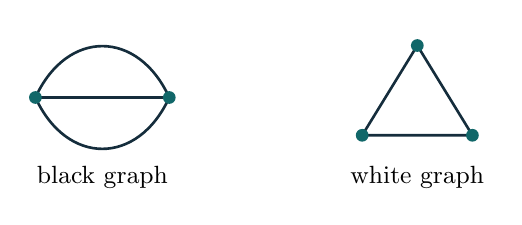
\begin{tikzpicture}[line width=0.95pt,line cap=round]
\begin{scope}
\draw[ink] (-.85,0) .. controls (-.45,.87) and (.45,.87) .. (.85,0);
\draw[ink] (-.85,0)--(.85,0);
\draw[ink] (-.85,0) .. controls (-.45,-.87) and (.45,-.87) .. (.85,0);
\fill[sea] (-.85,0) circle (2.3pt) (.85,0) circle (2.3pt);
\node[font=\small] at (0,-1.01) {black graph};
\end{scope}
\begin{scope}[shift={(4.0,0)}]
\draw[ink] (0,.66)--(-.70,-.48)--(.70,-.48)--cycle;
\fill[sea] (0,.66) circle (2.3pt) (-.70,-.48) circle (2.3pt) (.70,-.48) circle (2.3pt);
\node[font=\small] at (0,-1.01) {white graph};
\end{scope}
\end{tikzpicture}
\end{center}
\noindent For the standard positive trefoil all-$A$ smoothing leaves two circles; all-$B$ leaves three. Its black graph therefore has three parallel edges, and its plane dual is a triangle. Choosing any one black edge (or omitting any one white edge) gives a spanning tree. This recovers $|V(-1)|=3$ and makes the extreme bracket exponents $5$ and $-7$ visible from the two circle counts.

Let $P=t+t^3-t^4$ and $P^*(t)=P(t^{-1})$. The granny knot, its mirror,
and the square knot have polynomials $P^2,(P^*)^2,PP^*$, respectively:
they are the sums of two right trefoils, two left trefoils, and one of
each. Their degree intervals $[2,8],[-8,-2],[-3,3]$ separate all three.
Each knot has crossing number six, since a six-crossing sum diagram
exists and its Jones span in $t$ is six.

For the figure-eight knot use the closed three-braid
$(\sigma_1\sigma_2^{-1})^2$, with zero writhe. Set
$x=A^{-2}$, $y=A^2$, $e=e_1$, $f=e_2$. The bracket expansion of one
factor is $Q=I+xe+yf+ef$. The normalized closure evaluation
$\operatorname{tr}$ sends $I$ to $\delta^2$, $e,f$ to $\delta$ and
$ef,fe$ to $1$, by direct tracing. It is cyclic since the seam of a
stacked closed rectangle can be taken before or after either factor.
Expanding $Q^2$ and using the cap-cup identities gives
\[
 \operatorname{tr}(Q^2)
  =(1+x^2+y^2)\delta^2+4(x+y)\delta+5
  =A^8-A^4+1-A^{-4}+A^{-8}.
\]
Thus $V=t^2-t+1-t^{-1}+t^{-2}$ and four crossings are necessary and
sufficient (the closure permutation is a three-cycle). Its mirror
equivalence also has a finite witness. If $s=\sigma_1$, $u=\sigma_2$,
then $\Delta=sus=usu$ conjugates $s$ to $u$ and $u$ to $s$, by that
same braid relation. Conjugation therefore changes $(su^{-1})^2$ to
$(us^{-1})^2$. Cyclically permuting the latter gives $(s^{-1}u)^2$,
the mirror. For closed braids cyclic permutation slides the marked seam
around the annulus, and conjugation reduces to cyclic permutation and
adjacent inverse cancellation. These observations supply the moves;
equality of the two Laurent polynomials alone would not supply them.

\paragraph{Arithmetic implementation.}
A table of $4c$ half-edges, plus $z$ isolated circles, suffices. Boolean
reachability closure by $4c$ rounds computes the state components and
their least representatives. Every state has $1\le h\le H=2c+z$:
each non-isolated component uses at least two half-edges.
Allocate exponent slots from $-4c-2H$ through $4c+2H$ to include
normalization. The sum of absolute coefficients before cancellation is
bounded by $2^c 2^{H}$, since one state has coefficient norm
$2^{h-1}$. Powers of $\delta$ can be accumulated by shifted addition.
Spanning-tree selection needs one edge scan with bounded component
recomputation; counting trees needs at most $2^c$ subsets. Each proof
inducts on a mask fold, a crossing-change list of length at most $c$, a
tree-edge scan, or a move list with its given length. For the evaluation at one use a postorder fold over the ternary table of partially resolved states of the original diagram. For deletion--contraction fix the original vertex and edge bounds, allow deleted labels, and induct on the number of active edges with the induction predicate conjoined over all bounded incidence tables of the given size. Equalities of
polynomials mean bounded slot equalities, connectivity is a Boolean
matrix computation, and component counts use bounded sums. In particular
the minimal-crossing conclusion quantifies over a proposed alternative
diagram and an explicit move list. It does not require producing a
shortest list or deciding whether two arbitrary diagrams are equivalent.

\paragraph{Lean proof structure.}
Use $\mathtt{Nat}$ for mask and coded input, an offset coefficient vector for
$\mathtt{Laurent}$, and a finite array of mates for a boundary pairing.
Implement \texttt{stack} by bounded component/path tracing, returning
the new pairing and a loop count. Prove its gluing law by mapping each
path segment in the two-stage trace to its original edge list. For the
local tables it suffices to tabulate $I,e,f,ef,fe$ on six endpoints
and check the three cap-cup equations by computation. For adequacy,
first establish \texttt{switch\_merge} on two different cycle IDs and
\texttt{switch\_bound} on an arbitrary pair by cutting the two edges
and tracing the two resulting paths. Define \texttt{treeMask} by the
edge scan and maintain that the current forest partition equals
the cycle partition of the tree-switched state. Count face orbits and
use the checked Euler equality $a+d=c+2$. Finally reduce a
coefficient vector into four signed slots using $A^4=-1$; the tree
bijection identifies one slot with $\pm\tau$. Each bounded invariant is
suitable for quantifier-free induction after replacing list quantifiers
by Boolean scans.

The companion \texttt{jones\_states.py} directly enumerates braid states by
gluing the levels of the braid diagram. Its open-pairing checks retain
boundary information in moves II and III. Its closed computations test the
two-strand formula and both mirror choices through eleven crossings, the
figure-eight calculation, and the value and exponent grading on all 341
three-strand words of length at most four.

\section{An integral family of finite-type invariants}
\label{sec:finite-type}
A singular diagram with $m$ marked double points specifies $2^m$ ordinary diagrams by resolving each mark as a positive or negative crossing, keeping the strands and their arrows. Define its $m$th difference of an invariant as the sum over resolutions with sign $(-1)^{\#\text{negative resolutions}}$. A knot invariant has type at most $k$ if this difference is zero on every diagram with $k+1$ marks. This is the finite diagram form of the Vassiliev extension rule \cite{birmanlin}.

\begin{theorem}[Truncated Jones coefficients]\label{th:finite-type}
For each $k\ge0$ define the integer $v_k(D)=[h^k]F_D(1+h)$, where $F$ is the writhe-normalized bracket. The function $(k,D)\mapsto v_k(D)$ is primitive recursive. Each $v_k$ has type at most $k$. The invariant $v_2$ has type exactly two on knots; in this normalization its value is $-48$ on either trefoil and zero on the unknot.
\end{theorem}
\begin{proof}
Calculate in $R_k=\mathbb Z[h]/(h^{k+1})$, represented by $k+1$ signed slots. The inverse of $1+h$ there is $1-h+h^2-\cdots+(-h)^k$, by telescoping. Thus the substitution is a ring map on Laurent polynomials; its coefficients survive all moves by Section~\ref{sec:bracket}. Multiplication is truncated convolution, and signed powers of $1+h$ are computed by iteration using the indicated inverse for negative exponents.

Distribute the writhe normalization among the crossings, giving a crossing of sign $e$ an extra factor $(-A^3)^{-e}$. At a marked site the two crossing tensors are linear combinations of the \emph{same} two geometric pairings, with weights $A,A^{-1}$ interchanged, and their two normalizing factors as above. At $A=1$ both tensors have coefficient $-1$ on each pairing. Consequently, after $A=1+h$ the coefficient difference on each pairing is a multiple of $h$. Choose a boundary pairing at every site and expand the alternating sum. Its coefficient factors into the product of the local differences at the marked sites, times the common coefficients elsewhere. The closure loop count depends only on the selected pairings. Hence each summand contains $h^m$, and its coefficient of $h^k$ is zero if $m>k$. This is finite distributivity over $2^m$ sign masks, proved by folding one bit at a time. It proves the type upper bound directly over the integers.

The trefoil has $F=A^{-4}+A^{-12}-A^{-16}$. Modulo $h^3$ the coefficient of $h^2$ in $(1+h)^j$ for any integer $j$ is $j(j-1)/2$, by multiplying the truncated series forwards or backwards. Thus $v_2=10+78-136=-48$; on the mirror it is $6+66-120=-48$. On a circle $F=1$. Mark two of the three positive crossings of the standard two-braid trefoil. The four resolutions have exponents $3,1,1,-1$ after inverse cancellation. Each closure at $1$ or $-1$ is an unknot with a curl. Their second difference is therefore $-48$, proving that type at most one fails by a particular witness.
\end{proof}

The numerical distinction between two finite-type coefficients deserves emphasis: the theorem gives an upper bound on order for \emph{every} $k$, while its lower-bound example proves sharpness for $k=2$. Checking vanishing coefficients requires only the $k+1$ slots and the finite state sum, including when $k$ is an input rather than a fixed metatheoretic numeral.

\section{Wirtinger words and the Alexander polynomial}
\label{sec:alex}
A meridian label stays fixed along an overpass. On an underpass a label $x$ becomes $S_y(x)$ on crossing the normal of the oriented overpass, whose label is $y$. Choose the normal so that a positive downward crossing with the left strand over gives bottom colors $(S_x(y),x)$. Reading backwards uses $S_y^{-1}$. In this section we let the labels themselves be formal generators. We obtain invariants even where the sets they present are infinite, by recording finite substitutions and finite verifications of the relations. The classical background is the Wirtinger presentation and the first elementary ideal \cite{alexander,hiller,colorknots}.

\begin{lemma}[Eliminating local labels]\label{lem:eliminate}
Suppose $S_y$ is invertible, fixes $y$, and $S_z S_y=S_{S_z(y)}S_z$. If the inverse and these identities are witnessed by formal computations in the labels, either side of a Reidemeister replacement gives the same relations on the outside labels after explicitly eliminating the inside labels.
\end{lemma}
\begin{proof}
A variable appearing as $v=W$ with $W$ using the other variables can be removed by substituting $W$ and remembered for the inverse operation. In a crossing, start at either end of the underpass; the overpass keeps its label. At a curl with entry $a$ the new under label is $S_a^{\pm1}(a)=a$. If the returning overpass instead carries the unknown $b$, the equation $b=S_b^{\pm1}(a)$ gives $a=S_b^{\mp1}(b)=b$. In a bigon the lower strand is acted on by an operation and its inverse. In the triangle first name the top strand $z$, then propagate along the middle strand, then along the bottom one. Transport across the top sends the middle label $y$ to $A(y)$ with $A=S_z$ or $S_z^{-1}$. The two bottom computations agree because $A S_y^e=S_{A(y)}^e A$ for $e=1,-1$. The negative versions follow by inversion or substitution of $S_z^{-1}(y)$ in the given identity. This calculation can be read in either direction along each arc. All interior labels were solved for, so the two presentations reduce to identical boundary constraints in every orientation. Arbitrary outside relations are carried unchanged through these substitutions.
\end{proof}

\begin{theorem}[Wirtinger presentations]
Use one group generator for every arc between undercrossings, or one for a component with no undercrossings. At a crossing record the word relation $z=y^e x y^{-e}$ with $e=\pm1$ from the overpass normal. A move list gives explicit mutually inverse maps of the presented groups. The abelianization on a link of $r$ components is free abelian on its $r$ meridians. Mirroring preserves the isomorphism class of the group. Counting solutions in any supplied finite group table is a PR invariant.
\end{theorem}
\begin{proof}
One can equally put variables on all edge segments and impose equality across overpasses. In a group use $S_y(x)=yxy^{-1}$. Conjugation is invertible and preserves products and inverses; hence it commutes with conjugation by $y$ if the conjugating argument is transported to $S_z(y)$. Apply Lemma~\ref{lem:eliminate}. Each substitution yields words for images of generators, and substitution back gives the original words by a list of the same relation uses and free cancellations. Compose such lists along the movie. This is an entirely syntactic formulation: $u=v$ in a presentation means existence of a word-replacement certificate using the relators in contexts, free cancellations/insertions, and inverse words. Verification is bounded by the supplied code. In the abelianized presentation the crossing relation is simply $z=x$, so it identifies all arcs on a component. The map sending each arc to the corresponding standard basis vector in $\mathbb Z^r$ and its inverse choosing one representative per component give explicit inverse substitutions. For a mirror use the same overpasses with the ambient plane reflected, so the normal direction interchanges. Sending each generator to the inverse of its corresponding generator respects the reflected relations and squares to the identity. This reflected diagram gives the mirror as does switching all crossings (the two spatial reflections differ by an orientation-preserving half-turn). For a finite group of order $h$ test the relations on all $h^g$ assignments to $g$ generators. The local substitutions induce inverse bijections of solutions. The computation applies to any fixed union of conjugacy classes for the meridians as well, since propagation only conjugates them.
\end{proof}

For a trefoil a positive two-braid acts by $P(a,b)=(aba^{-1},a)$. The product $ab$ is fixed and $P^2$ conjugates both entries by $ab$, by cancellation. To close $P^3$ one needs its second entry $(ab)a(ab)^{-1}$ to equal $b$. Equality of the first then follows from the preserved product. Thus the trefoil has presentation
\[
 \langle a,b\mid aba=bab\rangle\ \simeq\ \langle u,v\mid u^2=v^3\rangle .
\]
Take $u=aba$, $v=ab$, so $u^2=(aba)(bab)=v^3$. Conversely $a=v^{-1}u$, $b=u^{-1}v^2$ give $ab=v$ and $aba=bab=u$. The transpositions $(12),(23)$ satisfy $aba=bab=(13)$ and generate the six permutations on three letters. This quotient is nonabelian, whereas every quotient of the one-generator unknot group is abelian. More explicitly, an alleged movie would convert this assignment to powers of a single permutation and then back, forcing its two entries to commute. No algorithm for equality of group words in an arbitrary presentation is involved. The classical identification with $\pi_1$ of the complement is the external Wirtinger theorem.

\subsection{An invariant from polynomial relations}
Put $R=\mathbb Z[t,t^{-1}]$. Use a generator for every segment and impose the two linear relations at a crossing: the over labels agree, and the under labels satisfy $z=t^e x+(1-t^e)y$. Give an isolated circle one free generator. The resulting row matrix $M$ has $g$ columns. We will use the greatest common divisor of its minors of size $g-1$, with the empty minor $1$. This is the diagrammatic Alexander polynomial up to multiplication by $\pm t^j$. The unreduced meridional coloring presentation has a free constant-color direction; the classical identification with covering-space homology concerns its reduced Alexander data.

\begin{lemma}[Minor calculus]
For any $j\ge0$, the common divisors of the minors of size $g-j$ are invariant under elementary row or column operations, insertion/deletion of a redundant relation, and adjoining a generator with a defining equation $v=W$. Minors of size at most zero generate the unit ideal; if the size exceeds the number of rows they generate the zero ideal. Indeed the corresponding ideals of minors agree.
\end{lemma}
\begin{proof}
A determinant is the alternating sum over permutations. Linearity in one row or column and cancellation of pairs when two rows agree follow directly by interchanging the selected entries. Thus adding a multiple of another row changes any minor by a multiple of another minor of the same size or by zero. The inverse operation gives the other containment. The same argument covers columns, a unit scaling, and adding a row already expressed as a linear combination of existing rows. To adjoin $v=W$, clear its defining row and column by these operations to get $\mathrm{diag}(M,1)$ with one more column. Its minors of the new size $k+1$, $k=g-j$, that use the last row and column are old $k$-minors. Those using exactly one vanish. Those using neither are $(k+1)$-minors of $M$, each a linear combination of $k$-minors by expansion. The size-zero convention covers $k\le0$. These arguments provide combinations witnessing both containments.
\end{proof}

\begin{theorem}[Alexander invariant and its specialization]
The first-minor gcd $\Delta_D$, taken up to $\pm t^j$, is invariant under oriented Reidemeister moves. For a knot it has a unique representative with least exponent zero and $\Delta_D(1)=1$. Mirroring sends the Laurent class to the class of $\Delta_D(t^{-1})$. A split diagram with two nonempty separated parts has zero first-minor gcd.
\end{theorem}
\begin{proof}
The affine actions $S_y(x)=tx+(1-t)y$ satisfy Lemma~\ref{lem:eliminate}: any affine map $A$ on the line gives $A S_y=S_{A(y)} A$. The substitutions and their inverses correspond precisely to adjoining or deleting defining equations. When the inner variables have been removed, the remaining crossing equations are equal as linear forms, up to rewriting by already imposed equalities and multiplication by units $t^e$. Such rewriting is elementary row addition or unit scaling. The minor calculus proves invariance, even of the whole family of determinantal ideals. A reflected planar drawing with the same overpass has the opposite normal, so $t$ is replaced by $t^{-1}$. In a split diagram each of the two blocks has row sum zero. Changing one column in each block to the sum of that block's columns produces two zero columns; hence every $(g-1)$-minor is zero.

For a knot, at $t=1$ the equations are exactly the differences of consecutive segment generators as one traverses the knot. For $g>1$ drop the final difference and one endpoint column. The remaining path matrix has determinant $\pm1$, by successive expansion at the path end. The $g=1$ case uses the empty minor. Thus there is a minor $m$ with $m(1)=\pm1$. The gcd divides it over the integral Laurent ring, so its value at $1$ is $\pm1$. Shifting the lowest exponent to zero and fixing its sign at $1$ gives the required normalization.
\end{proof}

\paragraph{A bounded gcd algorithm.}
Clear powers of $t$ separately in each nonzero minor so its least exponent is zero. Over $\mathbb Q[t]$, use long division and the Euclidean algorithm; degree drops at each nonzero remainder, so both loops use at most the starting degree plus two iterations per pair. Taking the primitive integral part of the last nonzero monic gcd and multiplying by the integer gcd of the contents of the nonzero inputs gives the integral gcd. If all minors vanish, return zero. For completeness, the product of primitive integer polynomials is primitive: if a prime $p$ divided every coefficient of the product, reducing modulo $p$ would give two nonzero factors with zero product, contrary to multiplication of their leading coefficients. A number $>1$ has a least divisor $>1$, prime by a bounded trial search. Consequently contents multiply, by factoring out the individual contents. Clearing rational denominators and comparing contents shows that a primitive divisor over $\mathbb Q[t]$ of an integral polynomial divides its primitive part over $\mathbb Z[t]$. Together with the two division identities for the Euclidean gcd, this proves the algorithm. The divisibility statement for any given candidate uses its code as a free parameter. The gcd has no factor $t$ since one shifted input already has nonzero constant term. The units of the Laurent ring are exactly $\pm t^j$ by the lowest and highest terms of a product.

For $g$ columns, minor enumeration uses bounded row/column masks and at most $g!$ permutations per determinant. Each matrix entry is a finite Laurent array, so a determinant has degree window at most $g$ times the input window after common clearing. Long division has a nested degree counter and ordinary rational coefficient operations, all PR. An arithmetic induction for polynomial division keeps $f=q h+r$ and a bound on the remaining degree; for Euclid it keeps the two successive division records (and optionally the two linear-combination multipliers) and the decreasing degree counter. The common-divisor argument takes a particular divisor as a free parameter, avoiding induction on an unbounded greatest-divisor property.

\subsection{The two-strand family and the figure-eight}
On a two-strand braid the action is now $P(x,y)=(x-t d,x)$ for $d=x-y$. Its new difference is $-td$. Set $S_m=\sum_{j=0}^{m-1}(-t)^j$. After $m$ positive crossings the change in the second entry is $S_m d$, and that in the first is $-t S_m d$. Eliminate the internal rows in the braid and use coordinates $(y,d)$. Closure imposes just $S_m d=0$, leaving $y$ free. The first minors have gcd $S_m$. In particular
\[
 \Delta_{T_{2,2k+1}}(t)=1-t+t^2-\cdots+t^{2k},\qquad
 |\Delta_{T_{2,2k+1}}(-1)|=2k+1 .
\]
This gives the determinant $3$ for the trefoil and $1$ for the unknot. At $t=-1$ the coloring relation recovers the Fox relation in Section~\ref{sec:fox}.

For the figure-eight, a block $Q=\sigma_1\sigma_2^{-1}$ sends $(x,y,z)$ to $((1-t)x+ty,z,t^{-1}x+(1-t^{-1})z)$. Put $y=x+d$, $z=x+e$. The first entry of $Q^2$ equals $x+t((1-t)d+e)$, so closure eliminates $e=(t-1)d$. The remaining two output-minus-input differences reduce to $t^{-1}(t^2-3t+1)d$ and $-t^{-2}(t^2-3t+1)d$. Thus the least-exponent-zero representative with value $1$ at $t=1$ is $-t^2+3t-1$. Its determinant is $5$. In particular the trefoil and figure-eight are inequivalent, as are their mirrors to each other across these two types.

\paragraph{The overview's Conway computation.}
For the odd two-strand knots the centered, value-one normalization is $t^{-k}S_{2k+1}$. For $k=1$ this is $t^{-1}-1+t=1+(t^{1/2}-t^{-1/2})^2$, giving the conventional Conway polynomial $1+z^2$ under $z=t^{1/2}-t^{-1/2}$. The same computation for the figure-eight gives $1-z^2$. Substitution is injective on $\mathbb Z[z]$, since the highest power in a nonzero polynomial contributes a unique top exponent in $t^{1/2}$. There is also a direct deduction of the entire two-strand recursion from the Conway axioms. Write $C_m$ for the Conway value of the standard closure, normalized by $C_1=1$. Applying the skein relation to a positive crossing gives $C_m=C_{m-2}+zC_{m-1}$ for $m\ge2$, since the switched pair cancels and the smoothing removes one crossing. The skein relation at a curl gives $zC_0=0$, hence $C_0=0$. Thus $C_2=z$, $C_3=1+z^2$, and $C_4=2z+z^3$. This final recurrence is a consequence of the stated Conway axioms; the diagrammatic Alexander-class construction and the explicit centered polynomials above were proved independently. We do not derive the globally sign-normalized Conway skein theorem for all links here.

\section{Linking, Gauss words and Brunnian links}
\label{sec:linking-surface}

For arithmetic statements involving planarity, take the supplied rational
polygonal realization of the diagram. Crossings are transverse intersections
in the interiors of segments. No vertex meets another strand and no three
strands meet. Label the components and direct each cyclic edge list.
Write $\epsilon(p)$ for the crossing sign, choosing the positive two-strand
braid generator to have sign $+1$ when both strands follow the braid.
Equivalently this is a fixed sign times
$\operatorname{sgn}\det(u_{\rm over},u_{\rm under})$ for the two
directed tangents. The fixed sign depends on the orientation convention
for the drawing plane and cancels in the argument below.

\begin{lemma}[Signed planar intersection]
\label{lem:rational-mixed}
For two closed oriented rational polygonal walks $P,Q$ in mutual general
position, the sum of $\operatorname{sgn}\det(u_P,u_Q)$ at their
intersections, counting pairs of passages, is zero. In particular their
number of intersections is even.
\end{lemma}
\begin{proof}
Choose a point $a$ avoiding the supporting lines of the edges of $P,Q$,
the lines from vertices of $P$ through vertices of $Q$, and the lines
through vertices of $P$ parallel to edges of $Q$. From $N$ forbidden lines
one obtains such an $a$ by testing $(j,j^2)$ for $0\leq j\leq2N$.
A line excludes at most two tests. For each successive pair $p_i,p_{i+1}$
use the directed boundary of the triangle $(a,p_i,p_{i+1})$.
For a counterclockwise triangle the summand is $+1$ when $Q$ enters
and $-1$ when it leaves, since its interior lies to the left of each edge.
The sum telescopes to zero along closed $Q$. One may split its edges at
the finitely many intersections and use the inside bits of the consecutive
open pieces. A clockwise triangle multiplies this identity by $-1$.
Adding the identities cancels each spoke in opposite directions and
leaves precisely the intersection sum for $P$. Equal positive and negative
counts give the parity assertion.
\end{proof}

\begin{theorem}[Three crossing formulas for linking]
For distinct components $i,j$, the signed sum $O_{ij}$ at crossings
where $i$ passes over $j$ equals $O_{ji}$. Their common value
$\ell_{ij}$ satisfies
\[
  \ell_{ij}=\ell_{ji}
  =\frac12\sum_{p\text{ between }i,j}\epsilon(p).
\]
It is invariant along every Reidemeister movie preserving the component
labels and orientations. Mirroring negates it. Reversing exactly one
of the two components negates it, and reversing both preserves it.
\end{theorem}
\begin{proof}
In the intersection sum ordered as $(i,j)$ the over-$i$ terms agree with
their crossing signs up to the fixed sign, and the over-$j$ terms have the
opposite comparison. Lemma~\ref{lem:rational-mixed} gives
$O_{ij}-O_{ji}=0$. A curl involves only one component. In a type II
bigon the same strand is upper at the two crossings and the directed
intersection signs are opposite. Indeed, following one side of the bigon
across the other strand enters and exits on opposite sides. Reversing
either orientation flips both local comparisons. In type III, each
pair of participating strands crosses once on either side, with the same
relative height, directions and crossing sign. These verifications also
apply when two of the participating strands belong to the same component.
An over/under switch reverses the determinant order. Reversing one tangent
changes its sign. The transformation laws follow term by term.
\end{proof}

Let $w$ be the sum of all crossing signs and $w_i$ the sum over crossings
of $i$ with itself. Thus
\[
  w=\sum_i w_i+2\sum_{i<j}\ell_{ij}.
\]
The same local proof leaves $w$ fixed in types II and III. A curl changes
it by its sign. Mirroring negates $w$ and reversing all components
preserves it. For any diagram, the number of crossings between $i,j$
is at least $2|\ell_{ij}|$. A change of such a crossing changes
$\ell_{ij}$ by exactly one in absolute value. A crossing change involving
another unordered pair, or a self-crossing, leaves it fixed. Consequently
every movie using ordinary moves and crossing changes to separate a
partition $S\mid T$ of the components into disjoint diagram boxes
uses at least $\sum_{i\in S,j\in T}|\ell_{ij}|$ crossing changes.
This follows from the triangle inequality at each step, since all these
entries vanish in the separated boxes.

\begin{corollary}[Even two-strand torus links]
For the closure of $\sigma_1^{2r}$, $r\in\mathbb Z$, the components with
their braid orientations have linking number $r$. The least crossing count
in its diagram-movie class is $2|r|$, and the least number of crossing
changes needed to obtain the two-component unlink is $|r|$.
In particular the Hopf link has crossing number two.
\end{corollary}
\begin{proof}
The strand permutation is the identity. Every one of the $2|r|$
crossings is between the two components and they have the same sign
when $r\ne0$. This realizes the crossing lower bound. Switch one letter
in each consecutive like-signed pair; each pair then cancels by type II.
The resulting empty two-braid closes to the unlink. The linking bound
gives the reverse inequality, including $r=0$.
\end{proof}

\begin{theorem}[The Dowker even--odd rule]
In a one-component plane diagram with $c$ crossings, label the $2c$
successive visits $1,\ldots,2c$ starting at any regular basepoint.
The two labels at every crossing have opposite parity. Hence in order
of the odd labels the partner labels are a permutation of $2,4,\ldots,2c$.
\end{theorem}
\begin{proof}
Cut the parametrizing circle at its two visits to a particular crossing.
Each of the two resulting arcs closes locally: its two ends lie on
different strands and hence at adjacent corners of a crossing box.
The two reconnections can be drawn separately along opposite sides of
that box. Between the two visits each self-crossing of the chosen arc
occurs twice and each crossing with the other arc occurs once. The
latter number is even by Lemma~\ref{lem:rational-mixed} applied to
the reconnected polygons. If the visits have labels $a<b$, their
difference is one more than this even total $b-a-1$. Each even visit
therefore partners one odd visit. Ordering by the latter yields the
claimed permutation; recording whether the even visit is under or over
provides the extra sign of a signed Dowker code.
\end{proof}

\begin{proposition}[The Borromean deletion test and failure of pairwise detection]
The standard Borromean closed braid $B=(\sigma_1\sigma_2^{-1})^3$ has
three components. Each two-component sublink is the unlink and all three
pairwise linking numbers vanish. The full link is distinct from the
three-component unlink under Reidemeister movies.
\end{proposition}
\begin{proof}
Label the top strands $1,2,3$. The unordered pairs exchanged successively
are $12,13,23,12,13,23$, with signs $+,-,+,-,+,-$. The final ordering
is $123$, so each strand closes to its own component. After deleting any
one component, the other two cross once positively and once negatively.
Their two-strand word reduces by one cancellation and their closure is an
unlink. To distinguish all three together, give the top strands Fox colors
$(a,b,c)$ modulo $q\ge2$. A positive letter sends the affected pair
$(x,y)$ to $(2x-y,x)$ and a negative letter to $(y,2y-x)$. A closure
coloring is exactly a fixed vector. Substituting the six letters gives
\[
 (M-I)\begin{pmatrix}a\\b\\c\end{pmatrix}
 =4\begin{pmatrix}2&-1&-1\\-1&0&1\\-3&1&2\end{pmatrix}
   \begin{pmatrix}a\\b\\c\end{pmatrix}.
\]
The second row and then the first give $4(c-a)=4(b-a)=0\pmod q$;
these conditions imply all three rows. Each difference has
$\gcd(4,q)$ choices, since $4x=0\pmod q$ means
$q/\gcd(4,q)$ divides $x$. Thus the color count is
$q\gcd(4,q)^2$. At $q=3$ this gives $3$, whereas the unlink has
$3^3=27$. The Reidemeister bijections for Fox colorings prove the
distinction. In particular, even the complete list of pairwise linking
numbers cannot detect all linking.
\end{proof}


\begin{corollary}[Six crossings are necessary for the Borromean rings]
The least crossing count in the Borromean diagram-movie class is six.
\end{corollary}
\begin{proof}
Use the bracket and span bound of Section~\ref{sec:bracket}. In the
six-letter braid above, the writhe is zero. Here is its complete state
count grouped by the number $b$ of $B$-pairings and the number $h$ of
circles. The rows are $b=0,\ldots,6$ and the columns are $h=1,2,3,4$:
\[
  \begin{pmatrix}
  0&0&0&1\\0&0&6&0\\0&15&0&0\\16&0&4&0\\
  0&15&0&0\\0&0&6&0\\0&0&0&1
  \end{pmatrix}.
\]
To reproduce each entry, trace three columns through seven horizontal
levels. At letter $j$ join each unaffected column to its successor.
Pair the two affected columns vertically for an $A$ at a positive
letter or a $B$ at a negative letter. Otherwise join the two upper
entries and join the two lower entries. Identify bottom and top and
count equivalence classes on the $21$ entries. Summing
$A^{6-2b}(-A^2-A^{-2})^{h-1}$ with the displayed multiplicities, and
putting $X=A^4$, gives
\[
 -X^3+3X^2-2X+4-2X^{-1}+3X^{-2}-X^{-3}.
\]
Its value at $X=-1$ is $16$. A disconnected shadow forces the bracket
to have a factor $-A^{-2}(A^4+1)$, by splitting its nonempty pieces
in the state sum. Hence every equivalent diagram has connected shadow.
The $A$-span is $24$, so the bound $\operatorname{span}_A\le4c$ gives
$c\ge6$. The braid attains equality.
\end{proof}

\section{A rational Seifert surface and its genus certificate}
\label{sec:seifert}
At a crossing there are two incoming and two outgoing corners. Each
through strand joins opposite corners, so the two incoming corners
are neighbors in cyclic order. Replace the crossing by the unique
noncrossing pairing joining incoming to outgoing. The result consists of
$s$ disjoint oriented polygonal circles, the \emph{Seifert circles}.
Isolated crossingless circles are included. The following elementary
capping lemma makes the geometric content of the disk-and-band construction
explicit.

\begin{lemma}[Planar polygon caps]
\label{lem:slab-cap}
There is a primitive recursive construction of a rational triangulated
disk bounded by a supplied simple rational polygon $P$. For finitely
many disjoint such polygons their planar disks have disjoint interiors
or are nested, and the strict containments are decidable.
\end{lemma}
\begin{proof}
Shear by $(x,y)\mapsto(x+hy,y)$ so that the vertices have distinct
first coordinates. Each vertex pair forbids at most one integer $h$.
Split the plane at these coordinates into vertical slabs. In an open slab,
sort the intersecting edges by height at the midpoint abscissa. This order
is constant within the slab, since edges do not cross. The gaps between
edges have alternating labels, starting with $0$ above the polygon.
Across an open piece of a slab wall the labels agree: at a vertex the
number of edges above changes by zero or two. Thus crossing any polygon
edge changes the label, and walking through a wall away from the polygon
preserves it. The label-one gaps are bounded triangles or trapezoids.

Here are the two connectivity facts needed about this subdivision. On a
small punctured neighborhood of a vertex, its two incident segments cut
the neighborhood into two sectors. The labels differ across the segments,
so the label-one sides of its consecutive edges meet through the same
sector. Walking the boundary in order therefore connects every edge's
label-one side to every other. Every label-one gap has a polygon edge
as its ceiling or floor, giving connectedness of the label-one cells by
wall adjacency. The same argument applies to the label-zero sides.
Every bounded label-zero gap touches such a side, and the outside gaps
join above, below or around an extreme vertex. Consequently every
label-zero point away from $P$ can be routed to the unbounded gap.
These statements concern finite cell adjacency. Near a vertex one can
take a square of radius less than its distances to nonincident segments
and other vertices.

Use the closures of the label-one gaps. Subdivide both copies of a
common wall at all polygon points on it. Triangulate a convex
trapezoid by a diagonal, with a single triangle when one end collapses.
To accommodate collinear marks on a side, split its incident triangle
from the opposite vertex, successively. All vertices of the resulting
triangles lie on $P$: even a wall endpoint in the middle of a polygon
edge lies on that edge. The dual graph, with one vertex per triangle
and one edge across each interior side, is connected by the preceding
cell argument and the triangulation within each gap.

Every interior side $e$ is a bridge in this graph. Join its endpoints
by either boundary subarc of $P$ to form a closed polygon with $e$.
If a dual path could bypass its dual edge, the bypass together with
that dual edge would give a closed walk through triangle interiors
crossing $e$ exactly once and disjoint from $P$. To draw the walk use
triangle interior points and side midpoints. At a crossed side join
nearby interior points directly so that its intersection is transverse
and interior to a segment. This contradicts the parity assertion of
Lemma~\ref{lem:rational-mixed}. The dual graph is thus a tree.
The triangulation can be assembled by attaching a triangle on a single
free side at each step along the tree. No extra identification at an
isolated corner is needed: around each boundary vertex the incident
triangles form one consecutive fan in its interior sector. Hence all
copies of that corner are already identified through shared sides.
A triangle attached on one entire boundary side to a disk gives a disk
(replace that side of the boundary by the other two), proving the claim.
The tree order itself is a disk certificate.

For disjoint polygon boundaries $P,Q$, the bit for $P$ is constant
along $Q$. If $Q$ has bit one, the exterior of $P$, together with its
boundary, has routes to infinity avoiding $Q$. These points are exterior
to $Q$; its disk therefore lies inside the disk of $P$. If each boundary
is exterior to the other, the bit for $Q$ is constant on the connected
interior of $P$ and is zero just inside its boundary, hence the disk
interiors are disjoint. Both bits cannot be one, by strict containment.
A wall or ray meeting a vertex is handled by its neighboring gap, or by
subdivision and an interior test point. Inverting the shear restores the
original rational coordinates.
\end{proof}

\begin{theorem}[Seifert construction with a boundary witness]
\label{thm:seifert-pl}
From a nonempty oriented rational plane link diagram with $c$ crossings,
$b$ components and $s$ Seifert circles, one constructs by primitive
recursion a rational embedded orientable triangulated surface whose
boundary projects to that same decorated diagram, up to subdivision.
It has $k$ connected components, where $k$ is the number of components
of the incidence graph of Seifert circles and crossing bands. Its Euler
characteristic and total handle genus $G$ satisfy
\[
  \chi=s-c,\qquad 2G=2k-b-s+c.
\]
In particular a knot diagram gives a connected surface of genus
$g_D=(1+c-s)/2$, an explicit upper bound for the spanning genus of the knot.
\end{theorem}

\begin{proof}
Fit disjoint rational parallelograms at the crossings, with corners
on the four strand ends. They can be chosen as the convex hull of
$p\pm t u,p\pm t v$ at a crossing $p$ of strands with directions
$u,v$. Take pairwise crossing distances, distances from crossings to
nonincident closed segments and to the endpoints of their incident
segments. Their positive squared distances have a rational minimum $m$
(append $1$ before taking minima). For a point and a segment the squared
distance is computed by projecting to its supporting line and clamping
the rational parameter to $[0,1]$. With $H$ the maximum of $1$ and
the $\ell^1$ norms of the directions, one may take
$t=\min(1,m)/(100H)$. Thus no unrelated pieces enter these
parallelograms. Their opposite sides used by the oriented smoothing
serve as the two attachment intervals. Outside them retain the input
segments. This gives the circles to which Lemma~\ref{lem:slab-cap}
applies.

Let $d(C)$ be the number of other disks strictly containing circle $C$,
and put its disk at height $-s+d(C)<0$. Connect its rim vertically
to the copy of $C$ at height zero using a triangulated wall of
rectangles. A containing disk lies below every contained one. The walls
of different circles have disjoint projections. A wall above an inner
disk never reaches the level of its containing cap, and disjoint
nonnested disks have disjoint projections. This proves pairwise
disjointness of the capped walls. Each is a disk with a collar and is
oriented to induce the specified direction on its upper boundary.

Use affine horizontal coordinates in each parallelogram so that the
attachment intervals are $x=-1$ and $x=1$ in the square $[-1,1]^2$.
The smoothing directs both intervals the same way in $y$. Here is a
specific half-twisted PL band. One boundary side visits
\[
 (-1,-1,0),\quad (0,0,1),\quad (1,1,0),
\]
and the other visits $(-1,1,0),(0,0,3),(1,-1,0)$.
Connect the two points in each column $x=-1,0,1$ and split each of the
two resulting four-sided patches along a diagonal into two triangles.
Within either half, one triangle projects onto a triangle of positive
area and the other onto a boundary segment of that triangle; their
intersection is precisely their common edge. The two halves meet only
on the middle vertical edge. The band meets the plane $z=0$ exactly
at its attaching ends. Its sides project to the original diagonals,
with the specified overpass obtained by interchanging the heights
$1,3$ when necessary. Because the order of the two side labels reverses
between the ends, the induced boundary directions of the rectangle
along both attachments point the same way in the drawing. Orient it
oppositely to the two disk boundary intervals. This consistently
orients the union. The patches occupy distinct boxes, and the rest of
the surface lies at $z\leq0$. The resulting list of triangles is an
embedded surface. Boundary subdivisions of the attachment intervals
are matched by splitting the corresponding band triangles from their
opposite corners. Its boundary follows the original crossing assignment
at every box and the original edges outside.

The disks and bands also give a purely finite computation of genus.
Initially there are $s$ disks with $s$ boundary circuits. Attaching a
rectangle on two disjoint intervals reduces the Euler characteristic
by one: after a common subdivision it contributes $1-2$ by
inclusion--exclusion for vertex, edge and face counts. The graph
components track the surface components. For a prefix of the bands let
$k',b',\chi'$ be the component, boundary and Euler counts. An oriented
band on two intervals of the same boundary circle splits that boundary
in two (trace the two complementary arcs after removing the intervals).
On two distinct boundary circles it merges them into one. In the latter
case the surface components also merge exactly when the intervals
belonged to distinct components. Starting with $G'=0$, increment $G'$
only for a band joining distinct boundary circles of the same component.
These three updates preserve
\[
                      2G'=2k'-b'-\chi'.
\]
They are also the handle description of orientable genus: a band on
one boundary splits a collar into a pair of pants; a band joining two
boundaries in one connected surface makes a handle, merging those
boundaries. Equivalently the displayed Euler relation computes total
genus for an orientable surface with boundary. At completion the
boundary circuits trace the diagram and number $b$. Every component of
a disk-and-band surface has boundary, by the same updates, so $b=1$
forces $k=1$. This proves all the formulas.
\end{proof}

\begin{corollary}[Bounds and operations]
A knot diagram with $c$ crossings bounds a surface of genus at most
$\lfloor c/2\rfloor$. For a connected sum made at regular arcs of two
separate oriented knot diagrams, the surface genus of the resulting
diagram is $g_{D\#E}=g_D+g_E$. Mirroring preserves $g_D$. For $p,q\ge1$,
the usual closure of $(\sigma_1\cdots\sigma_{p-1})^q$ has
$\gcd(p,q)$ components and a connected spanning surface of genus
\[
   \frac{2-\gcd(p,q)-p+(p-1)q}{2}.
\]
For coprime $p,q$ this gives the knot-genus upper bound
$(p-1)(q-1)/2$.
\end{corollary}
\begin{proof}
Use $s\ge1$ in the knot formula. In a connected sum, smoothing all
crossings on either side leaves exactly the two marked Seifert circles
spliced into one, so the crossing counts add and the circle counts add
with a subtraction of one. A mirror changes heights without changing
the oriented smoothing. For the displayed braid, with all strands
oriented along the braid, smoothing leaves all $p$ columns vertical and
each closes to its own circle. There are $(p-1)q$ crossing bands.
The incidence graph contains the path through adjacent columns and is
connected (also for $p=1$). The permutation of one block rotates the
$p$ labels by one, up to reverse convention. Its $q$th power has
$\gcd(p,q)$ orbits, since the subgroup of residues generated by $q$
consists of the multiples of $\gcd(p,q)$ modulo $p$, by the Euclidean
algorithm. Substitute these counts. Each upper bound is witnessed by the
constructed surface. Minimality among spanning surfaces would require a
lower bound and is not used in the construction.
\end{proof}

\paragraph{Arithmetic and Lean implementation.}
The planar-intersection loop stores the two signed counts and the current
triangle-inside bit. Its induction invariant is that the signed prefix
equals the final minus initial bit, multiplied by the triangle orientation.
For a polygon with $n$ vertices the shear has index at most $n(n-1)/2$.
There are at most $n+1$ slabs and at most $n+1$ gaps per slab.
Each slab wall has at most $n$ intersections with polygon edges plus
its vertex. Thus $10(n+1)^3$ suffices for the triangles of a single cap
and their intervening wall subdivisions. Connected components of a graph
with $v$ vertices may be computed by $v$ iterations of adding all
neighbors to a bit vector. The invariant says that its bits are exactly
the endpoints of walks of length at most the stage; walk certificates can
be bounded by $(v+1)^{v+1}$ for these stages. A cycle or bypass can be
shortened to a simple one by deleting repeated-vertex portions, with at
most $v+1$ successive retained vertices. Every instance of connectivity
in the cap proof uses these finite adjacency tests. The triangle-tree
gluing order gives local side and vertex fan checks. The depth list is
an $s$-by-$s$ table of ray parities, and the $c$ band additions carry
the equality $2G'=2k'-b'-\chi'$ as a signed-integer equality at every
prefix. There are at most $b+c$ Seifert circles, since each smoothing
changes the number of circuits by one in absolute value. All scalar
geometry uses rational determinants, additions, products and divisions
with nonzero denominators checked before use.

For Lean, implement a closed walk as a cyclic vertex array, a triangle
as a triple of rational pairs, and a surface as a list of rational
spatial triangles with oriented edge incidences. First prove triangle
entry/exit telescoping, then spoke cancellation and the signed crossing
identities. Encode a slab cell by its two adjacent abscissas and its
ordered floor/ceiling edges. The label is its vertical index modulo two;
prove wall agreement by inspecting the two edges at the wall vertex.
Prove the tree claim by converting a simple dual cycle into the rational
polygon used in Lemma~\ref{lem:slab-cap}. Independently encode each
disk rim by a cyclic word in its marked intervals. On band addition,
split a word at two marks or splice two words, removing the attaching
intervals and inserting the long band sides. The local cases above
prove the genus recurrence by induction on the word of bands.
Relate this combinatorial boundary to the triangle boundary by checking
the single two-patch band and the capped-wall template, then concatenate
the incidences. For object-theory induction, equality of arrays,
validity of all incidences and correctness of all bounded labels are
Boolean folds. This leaves only quantifier-free induction with the
input code as a free parameter.

\section{Finite tabulation and the first crossing number}
\label{sec:tabulation}

\begin{proposition}[A finite list of diagram codes]
For $c\ge1$, all oriented one-component planar diagrams with $c$
crossings, up to subdivided planar redraw, admit at most
\[
                         (c+2)4^c c!
\]
marked codes. Consequently there are finitely many diagrammatic knot
types admitting at most $n$ crossings. More precisely one may bound their
number by $1+\sum_{c=1}^{n}(c+2)4^cc!$.
\end{proposition}
\begin{proof}
Start just before any crossing visit, traverse the knot, and number visits
$1,\ldots,2c$. The Dowker even--odd rule proved above pairs the odd visits
bijectively with the even visits. Record that permutation of $c$ symbols.
On each pair record which visit goes over and the sign of the crossing.
This gives four choices per pair. There are $c+2$ possible exterior
faces on the connected sphere map, by Euler's formula. Mark the exterior
face by its index when face orbits are sorted by least dart.

The traversal tells which leaving dart joins which next arriving dart.
At a crossing of visits $i,j$, their incoming and outgoing darts are
opposite in pairs. Of the two possible oriented cyclic orders of these
four named darts, precisely one has the recorded crossing sign for the
recorded overpass. Thus the code recovers the oriented rotation table,
the edge pairing, and the overpass and orientation data. Successive
cyclic predecessors (or successors with the other fixed convention)
after edge reversal trace the faces. Discard codes with an invalid
permutation, face index, or Euler count. The argument only requires
that every diagram is represented. Distinct codes may describe the same
knot.

Here is why subdivision coordinates add no multiplicity to a fixed code.
Take disjoint small polygonal disks about the crossings and narrow strips
along the intervening arcs. Their cell patterns are prescribed by the
rotation table. Subdivide strip lengths on both drawings to match, and
triangulate their rectangular pieces in matching order, keeping the
diagram as center lines. The remaining bounded regions are disks with
simple polygon boundaries: thickening a spanning tree gives a disk and
inserting each remaining edge splits the corresponding complementary
disk in the sphere. For the marked exterior face use a large bounding
polygon; the extra region between its boundary and the outside boundary
of the thickening is an annulus. A narrow strip from one matched marked
point of the inner boundary to the outside box cuts this annulus to a
disk. Such a polygonal path can be drawn along the exterior collar to an
extreme vertex and then out along a supporting ray. The pieces can all
be taken rational: at each disjointness requirement take a positive
rational clearance smaller than the finitely many relevant separations.
For disjoint rational segments the squared separation is computed by
testing the endpoint-to-segment projections, clamped to the segment,
in both directions. For a squared separation $q>0$, half of
$\min(1,q)$ is a valid strict clearance. Direction and angular margins
at a vertex use the finite list of nonzero rational determinants.

Two polygonal disks with corresponding boundary vertices have compatible
triangulated subdivisions. To see this, triangulate each polygon by
diagonals. A short constructive diagonal argument is as follows. Remove
collinear subdivision points temporarily. Choose a strictly convex
vertex $v$ (one maximizing a generic linear functional suffices), with
neighbors $u,w$. If the closed triangle $uvw$ contains no further
vertex, $uw$ cuts off an ear, unless the polygon is already a triangle.
Otherwise join $v$ to a further vertex of this triangle farthest from
the line $uw$. The open segment so obtained has greater height above
$uw$ than any such further vertex. An unrelated polygon edge could only
enter the triangle through its base or end in the triangle, since it
cannot cross $vu,vw$. Hence it cannot cross that open segment.
The segment starts inside at the convex corner, and so is an interior
diagonal. Repeat on the smaller polygons and reinsert all boundary
subdivision points. Transport each triangulation to the same strictly
convex rational polygon with the matched boundary order (points
$(i,i^2)$ in increasing order, closed by the chord between the extreme
points, suffice). There the two triangulations overlay in convex cells;
triangulate those cells and pull the refinements back by the respective
rational affine maps on triangles. This gives the common triangulations
required for the redraw certificate. Together the matched disks, strips,
and exterior pieces give the claimed redraw.

Enumerating permutations, bit choices, and marked faces is bounded; a
coarser $c^c$-entry scan also suffices to enumerate the permutations for
$c\ge1$. The bound $c!$ follows by successively recording the rank of the
partner among the remaining even positions. The arithmetic statement of
finiteness is the finite coding and collision principle: in any supplied
list of knot diagrams with the indicated crossing cap and length greater
than the bound, two have identical positive-crossing codes and a redraw
witness, or two have zero crossings. Pigeonhole follows by counting
filled slots in a bounded Boolean array. Every oriented simple polygon
redraws to a triangle of matching orientation by the disk and exterior
construction. The two orientations of the unknot have a short move
witness. Orient the bow-tie polygon with successive vertices
$(-1,-1),(1,1),(-1,1),(1,-1)$ and choose either overpass at its double
point. Its upper and lower triangular lobes have opposite orientations.
Deleting one empty lobe or the other gives the two orientations of a
simple polygon. This justifies the one zero-crossing slot for knot types.
\end{proof}

\begin{theorem}[The smallest crossing number of a nontrivial knot is three]
Every knot diagram having one or two crossings admits a sequence of
type I deletions and planar redraws to a crossing-free diagram. The
trefoil realizes three and is nontrivial.
\end{theorem}
\begin{proof}
At two crossings the cyclic word of visits uses letters $A,B$ twice
each. The interlaced order $ABAB$ would pair two odd visits, contrary
to the even--odd rule. Up to cyclic shift and relabeling the word is
therefore $AABB$. The subarc between consecutive visits to $A$, closed
at its crossing, is a simple polygonal lobe. The analogous $B$-lobe is
disjoint from it. At the base of a lobe its two rays belong to different
passages and are adjacent in the cyclic order. The remainder of the knot
away from that base is a connected arc, so it lies entirely on one side
of the lobe. Choose a lobe whose bounded interior does not contain the
other lobe, by choosing the inner one if they are nested. Its interior
then misses the whole remainder of the diagram. It is an empty monogon.
A thin disk neighborhood of the lobe together with its empty interior,
extended slightly past the crossing, therefore has exactly the type I
curl pattern; the overpass choice permits one of the two type I
deletions. The polygon triangulation construction above supplies the local
redraw when the lobe has many subdivision vertices.

At a single crossing there are two such lobes, now meeting only at
their common base. Away from the base each lies entirely on one side
of the other. At least one bounded interior is empty of the other lobe:
if one contains the other away from their common point, its own boundary
away from that point is exterior to the contained lobe. This is also the
disk separation test on the two simple polygons. Delete the empty lobe
as before. The resulting crossing-free diagram represents the unknot.
The closed positive braid $\sigma_1^3$ has three crossings and Jones
polynomial $t+t^3-t^4\ne1$, as calculated in
Section~\ref{sec:bracket}. This proves both bounds.
\end{proof}

\section{Lean formalization and object-theory obligations}
\label{sec:lean}
A host theorem such as a divisibility criterion is a Lean proposition about integers. An object derivation is a term whose conclusion is a formula in a specified formal calculus. Both can be kernel-checked. The files have the following verification status.
\begin{center}\small
\renewcommand{\arraystretch}{1.20}
\begin{tabularx}{\linewidth}{@{}p{.237\linewidth}p{.19\linewidth}X@{}}
\toprule File in \texttt{lean/}& Verification & Scope\\\midrule
\texttt{EquationalFox.lean} & Lean 4.32.0 & Object derivations in the additive equational fragment: the three universal Fox identities, with signed inputs encoded as pairs.\\
\texttt{Fox.lean} & Lean 4.32.0 & Integer and modular local identities, signed two-braid powers and their closure condition; both rational-tangle closure criteria for arbitrary construction words.\\
\texttt{SurfaceCore.lean} & Lean 4.32.0 & Modular fixed rows of the Borromean braid; the Euler/genus invariant for every finite sequence of specified band cases.\\
\texttt{DiagramCore.lean} & Lean 4.32.0 & Executable pairing, state-circle and color-count definitions; closed evaluations on a curl, circle and braid examples.\\
\texttt{LocalIPRA.lean} & Unbuilt integration source & Targets ProveIt's actual \texttt{Prf PRAAx}, with open integer equalities and a closed six-variable Fox type III formula. Its imports include the repository's ring tactic and Mathlib.\\\bottomrule
\end{tabularx}
\end{center}
The four standalone files were run with Lean 4.32.0 and its standard library. The ProveIt integration dependencies were unavailable in the build environment. The full crossing-minimality, geometry, and knot-invariant theorems remain human proofs with the object-theory implementation plan below. The Python programs check enumerations, sample inputs, and in some cases entire supplied move lists. The archive README lists their individual checks.

\subsection{A checked equational derivation}
In \texttt{EquationalFox.lean}, terms are variables, zero, successor and addition. A derivation $D(\Gamma,a,b)$ derives one equation from a list of equation hypotheses. Its constructors are equality and congruence rules, the two defining equations of addition recursive on its second input, instantiation of an assumption-free schematic derivation, and equation induction. The last rule takes $a[0]=b[0]$ and, from the single hypothesis $a[i]=b[i]$, a derivation of $a[Si]=b[Si]$. Its conclusion has $i$ free, with universal closure understood. All other variables are parameters.

Each constructor has a direct iPRA interpretation. Interpret $D(\Gamma,a,b)$ as intuitionistic derivability of $a=b$ in the translations of $\Gamma$. Take an ambient context large enough for the free indices in the given derivation. Reflexivity is an equality rule, symmetry/transitivity and congruences follow by substitution. The recursion axioms specialize \texttt{PRA.precZero} and \texttt{PRA.precSucc} (exchange the arguments to obtain recursion on the second). An assumption-free derivation may be universally closed, instantiated and weakened. In equation induction rename the finitely many parameters so the induction variable is fresh for the empty external context. Apply \texttt{PRA.qfInd} to the translated equality, then specialize its universal conclusion to the original variable. Together these instructions give the rule-by-rule interpretation in ordinary iPRA. The separate ProveIt script demonstrates the intended destination.

The checked file derives $0+x=x$, $Sx+y=S(x+y)$, commutativity, and associativity from the two recursion equations. It forms the \emph{metatheoretic} quotient of terms by provable equality. Addition on that quotient is associative and commutative by the preceding derivations. Normalization for these two laws proves equality of classes, and exactness of the quotient returns an object derivation. For $x=(x^+,x^-)$, Fox reflection has pair
\[
  (y^++y^++x^-,\ y^-+y^-+x^+).
\]
Equality of signed pairs is translated to a single equation of natural terms by cross-addition. The Lean results are schematic object proofs before reduction modulo $n$. In particular \texttt{foxTriangle} has Lean's axiom report \texttt{[propext, Quot.sound]} for the metatheory. Its conclusion is derivability using the displayed rules for $D$.

\subsection{From the finite algorithms to \texttt{Prf PRAAx}}
At the revision in the bibliography, \texttt{PR k} has constructors zero, successor, projection, composition, and \texttt{prec}. Terms \texttt{PTm n} have variable and application constructors. The defining recursion uses $(i,\mathrm{previous},\mathrm{parameters})$ for the step arguments. Encode a loop starting with $a(x)$ and updating by $b(i,s,x)$ as the symbol $\operatorname{prec}(a,b)$. To run for $L(x)$ steps, compose it with $(L(x),x)$. To run several registers together put their tuple in $s$ and use projections in $b$. Expand this program syntax separately for each fixed algorithm in the paper. Use \texttt{Fm PTm} for formulas and the sequent $[]\mathrel{\vdash_{\rm PRAAx}}\forall\vec x\,\phi$ as the target.

For example, let $V$ be a numerical diagram validator, $P(D,E,p)$ the movie Boolean, and $F(D)$ the normalized polynomial code. The Jones invariance target has matrix
\[
 V(D)=1\ \land\ V(E)=1\ \land\ P(D,E,p)=1
      \ \longrightarrow\ F(D)=F(E).
\]
Table trimming makes the last equality numerical. A chosen coefficient slot may be an additional free parameter; a bounded conjunction covers any required range of slots. In an object proof for movie prefixes keep the full $p$ fixed, as in Lemma~\ref{lem:interface}. For a construction the target concludes $\operatorname{Check}(D,\operatorname{Build}(D))=1$, giving an existential corollary with $\operatorname{Build}(D)$ as its witness.

\begin{center}\small
\renewcommand{\arraystretch}{1.19}
\begin{tabularx}{\linewidth}{@{}p{.21\linewidth}X@{}}
\toprule Implementation stage & Lemmas needed for the object derivation\\\midrule
Codes and arithmetic & Prove lookup/update, bounded flags and prefix counts. Reuse the repository's signed pairs, division/remainder, gcd and bounded sums. Use equality substitution for modular operations.\\
Input and moves & Encode polygon vertices, segment tests and dart tables. Verify redraw incidences, local disk templates, certificate reversal, concatenation, and bounded path tracing. Prove transport along movies by prefix induction.\\
Rational geometry & Verify linear elimination, leading terms, root factorization and grid avoidance. For the cone check pairs of edges, then induct on the remaining fan. For the ribbon and Seifert constructions use pairwise triangle-incidence tests and disk certificates.\\
Colors and words & Use the three local identities to construct the extension tables. Count both projections of their graphs. Prove the braid difference invariant, the orbit enumeration and the changing-crossing kernel bounds. Induct on the number of trefoil summands.\\
Bracket and finite type & Build the state-pairing tables; verify local composition and closure. Maintain the forest partition and extremal degree inequalities under smoothing changes. In the signed state sum, after $j$ marked sites the first $j$ coefficient slots vanish.\\
Group and Alexander & Define word substitutions and their proof certificates. For linear relations use signed Laurent arrays, determinant expansion, row replacement and unit-pivot elimination. Record each nonzero remainder with its division identity.\\
Surfaces and tabulation & Derive polygon parity from triangle-entry counts, then cap adjacency, disk shellings, marked rim splices and the band invariant. Recover cyclic orders and face walks. Count the occupied encoding slots.\\\bottomrule
\end{tabularx}
\end{center}

For search claims, quantify over $p$ after proving the assertion for an arbitrary movie code. For connectedness on $v$ darts, at the $j$th adjacency iteration keep the Boolean array for endpoints reachable in at most $j$ steps; witnesses use at most $v+1$ base-$(v+1)$ digits up to the final pass. For a group certificate that grows under substitution, the new word length is at most the old length times the maximal image length. Iterate this bound along a fixed move list to obtain a PR length bound even for expanded certificates.

\paragraph{Induction over families of subproblems.}
For the bracket recursion at $A=1$, hold the original diagram fixed. A partial resolution is a word of $c$ ternary digits (keep the crossing, choose $A$, choose $B$). Induct on $j$ using the bounded conjunction of the desired identities for every partial resolution with at most $j$ live crossings. At the successor, its two children have one fewer live crossing. For Tutte deletion and contraction, order the original edges and record a deletion, contraction, or untouched bit-pair per edge; freeze isolated-vertex labels and canonicalize blocks by least representatives. Equivalently use the actual branching tree of depth at most $c$ on the least remaining edge, computed on all decision words of length at most $c$. Aggregate all nodes at a given remaining height into one Boolean. For ear splitting or disk shelling the nodes are sublists of the supplied finite triangulation or cyclic vertex list. Coding the list of subproblems before induction is what licenses these diagram-wide arguments with quantifier-free induction.

\paragraph{Further research questions.}
Can one convert a single rational spatial triangle move to a planar Reidemeister movie with a numerical bound in terms of the input charts, and compose these bounds without repeatedly changing projection? This would bring more of the classical Reidemeister theorem inside the object theory. A second target is a derivation identifying the Alexander first-minor gcd with the determinant of a Seifert pairing for every surface certificate. It would turn the explicit spanning surfaces here into sharp genus results when the polynomial has matching degree. A third is to formalize the reduced alternating crossing theorem as a \texttt{Prf PRAAx} endpoint using the finite forests in Section~\ref{sec:bracket}.

\section{Correspondence with the source articles}
\label{sec:scope}
The scope is the mathematical content of the requested \wiki{Knot_theory}{\emph{Knot theory} overview} and its directly linked topics. The table groups the source statements that have arithmetic counterparts here. The rational-tangle, torus-family and graph-polynomial results develop the relevant linked topics beyond the examples in the overview.
\begin{center}\small
\renewcommand{\arraystretch}{1.17}
\begin{tabularx}{\linewidth}{@{}p{.34\linewidth}X@{}}
\toprule Starting topic or linked article & Result in this report\\\midrule
Knot diagrams; \wiki{Reidemeister_move}{Reidemeister move}; \wiki{Unknotting_problem}{unknotting problem} & Regular projections, diagram lifts, move witnesses, bounded certificate search, and an explicit descending unknotting construction. Sections 1--3.\\
Higher dimensions; \wiki{Ribbon_knot}{ribbon knot}; \wiki{Slice_knot}{slice knot} & Every rational polygon in four-space reduces to a triangle. A marked rational ribbon disk lifts to a properly embedded slice disk. Section~\ref{sec:geometry}.\\
\wiki{Knot_sum}{Knot sum}; \wiki{Tricolorability}{tricolorability}; \wiki{Tangle_(knot_theory)}{tangles} & Sum laws, Fox coloring counts, torus knots, rational tangle closure tests, and the exact crossing-change cost of trefoil sums. Sections~\ref{sec:sums}--\ref{sec:fox}.\\
\wiki{Jones_polynomial}{Jones polynomial}; \wiki{Skein_relation}{skein relation}; alternating diagrams and Tait's crossing-number conjecture & The normalized bracket, mirror and sum laws, Tutte specialization, adequacy and the minimal-crossing theorem. Section~\ref{sec:bracket}.\\
\wiki{Vassiliev_invariant}{Vassiliev invariants} & Integer finite-type coefficients at every order; an explicit invariant of exact order two. Section~\ref{sec:finite-type}.\\
\wiki{Knot_group}{Knot group}; \wiki{Alexander_polynomial}{Alexander polynomial}; Alexander--Conway polynomial & Finite presentation transports, abelianization, gcd of first minors, family computations and the overview's trefoil computation. Section~\ref{sec:alex}.\\
\wiki{Trefoil_knot}{Trefoil}; \wiki{Hopf_link}{Hopf link}; \wiki{Borromean_rings}{Borromean rings}; mirror image & Explicit distinctions, chirality or mirror equivalence in worked examples, deletion certificates and exact crossing counts. Sections~\ref{sec:fox}--\ref{sec:linking-surface}.\\
\wiki{Link_(knot_theory)}{Links}; linking number; spanning surfaces & Signed crossing formulas; an embedded mesh, Euler characteristic and genus witness for an arbitrary oriented polygonal diagram. Sections~\ref{sec:linking-surface}--\ref{sec:seifert}.\\
\wiki{Dowker_notation}{Dowker--Thistlethwaite notation}; Gauss codes; \wiki{Knot_tabulation}{knot tabulation} & Even--odd pairing, an explicit factorial bound on diagram codes, and the first possible nontrivial crossing number. Sections~\ref{sec:linking-surface} and~\ref{sec:tabulation}.\\\bottomrule
\end{tabularx}
\end{center}

Classical knot recognition without a supplied certificate, uniqueness of prime decomposition, geometrization of knot complements, general smooth high-dimensional classifications, and the multiplication of knots described in the overview require additional ideas beyond this report. No unprovability claim about iPRA follows from these omissions. The proof of the first Tait conjecture here concerns crossing minimality; the flyping theorem is a different statement. The surface theorem constructs an upper bound on minimal genus. The Conway recurrence is used with its normalization explicitly stated.

\clearpage
\begin{thebibliography}{10}
\bibitem{overview} \emph{Knot theory}, Wikipedia, with the article links above. \url{https://en.wikipedia.org/wiki/Knot_theory}.
\bibitem{proveit} V.~Reshetnikov and contributors, \emph{ProveIt}, revision \href{https://github.com/VladimirReshetnikov/ProveIt/commit/6d03f3643ebb91a6243eb1e35e7599b388197786}{\texttt{6d03f3643ebb}}. See the \repo{Logic/PrimitiveRecursiveArithmetic/README.md}{iPRA overview}, \repo{Logic/PrimitiveRecursiveArithmetic/ConciseIPRA/Lean/ConciseIPRA/PR.lean}{object syntax and induction}, and \repo{Logic/PrimitiveRecursiveArithmetic/Derivations/Lean/IPRADerivations/Core/Tactic.lean}{integer derivation tactics}. The research packets and checked library components have separate verification statuses.
\bibitem{validator} \emph{ProveIt}, same revision. \repo{Topology/UnknotRecognition/reports/06/unknot/diagram.py}{Planar-diagram validator}, including its dart convention, face permutation and spherical Euler test.
\bibitem{rei} K.~Reidemeister, \emph{Elementare Begr\"undung der Knotentheorie}, Abh. Math. Sem. Univ. Hamburg \textbf{5} (1927), 24--32. \href{https://doi.org/10.1007/BF02952507}{doi:10.1007/BF02952507}.
\bibitem{kauffman} L.~H.~Kauffman, \emph{State models and the Jones polynomial}, Topology \textbf{26} (1987), 395--407. \href{https://webhomes.maths.ed.ac.uk/~v1ranick/papers/kauffmanjones.pdf}{Paper}.
\bibitem{alexander} J.~W.~Alexander, \emph{Topological invariants of knots and links}, Trans. Amer. Math. Soc. \textbf{30} (1928), 275--306. \href{https://homepages.math.uic.edu/~kauffman/Alex.pdf}{Paper}.
\bibitem{hiller} S.~Fushida-Hardy, \emph{Knot theory}, Stanford reading-course notes, especially Chapters 5, 6 and 9. \href{https://stanford.edu/~sfh/knot.pdf}{Notes}.
\bibitem{colorknots} A.~B.~K{\i}l{\i}\c{c}, A.~Nijsten, R.~Pellikaan and A.~Ravagnani, \emph{Knot theory and error-correcting codes}, Des. Codes Cryptogr. \textbf{93} (2025), 3029--3068. \href{https://arxiv.org/abs/2307.14882}{arXiv:2307.14882}.
\bibitem{birmanlin} J.~S.~Birman and X.-S.~Lin, \emph{Knot polynomials and Vassiliev's invariants}, Invent. Math. \textbf{111} (1993), 225--270. \href{https://www.math.columbia.edu/~jb/v-inv.-knot-poly.pdf}{Paper}.
\bibitem{prz} J.~H.~Przytycki, \emph{3-coloring and other elementary invariants of knots}. \href{https://arxiv.org/abs/math/0608172}{arXiv:math/0608172}.
\bibitem{shimizu} A.~Shimizu, \emph{The warping degree of a knot diagram}. \href{https://arxiv.org/abs/0809.1334}{arXiv:0809.1334}.
\end{thebibliography}

\end{document}
